\documentclass[sigconf,review,anonymous]{acmart}\settopmatter{printfolios=true,printccs=false,printacmref=false}


\usepackage{mathtools}
\usepackage[T1]{fontenc}
\usepackage{textcomp}
\usepackage{algpseudocode}
\usepackage{algorithm}
\usepackage{xcolor}
\usepackage{bytefield}
\usepackage{lipsum}
\usepackage{float}
\usepackage{setspace}
\usepackage{url}
\usepackage{caption}
\usepackage{graphicx}
\usepackage{multirow}
\usepackage{soul}
\usepackage{balance}

\usepackage{array}
\usepackage[bottom]{footmisc}
\raggedbottom
\newcolumntype{P}[1]{>{\centering\arraybackslash}p{#1}}

\acmConference[SC'19]{}{2019}{U.S}
\acmYear{2019}
\acmISBN{} % \acmISBN{978-x-xxxx-xxxx-x/YY/MM}
\acmDOI{} % \acmDOI{10.1145/nnnnnnn.nnnnnnn}
\startPage{1}


%\newcommand{\comments}[1]{\textcolor{blue}{[#1]}}
%\newcommand{\removetext}[1]{\textcolor{blue}{\st{#1}}}
%\newcommand{\rephrased}[1]{\textcolor{magenta}{#1}}
%\newcommand{\added}[1]{\textcolor{violet}{#1}}
%
%\usepackage{color, colortbl}
%\definecolor{Gray}{gray}{0.85}
%\definecolor{LightCyan}{rgb}{0.88,1,1}
% Some very useful LaTeX packages include:
% (uncomment the ones you want to load)

% ALGORITHM RENEWCOMMAND
%\renewcommand{\algorithmicendfor}{\algorithmicend}
%\renewcommand{\algorithmicendwhile}{\algorithmicend}
%\renewcommand{\algorithmicendif}{\algorithmicend}
%\renewcommand{\algorithmicdo}{}
%\renewcommand{\algorithmicthen}{}
%\floatname{algorithm}{\textnormal{Algorithm}}
%\restylefloat{algorithm}
%\renewcommand{\thealgorithm}{\textnormal{\Roman{algorithm}}}
%\newcommand{\algorithmname}{Algorithm}


% *** MISC UTILITY PACKAGES ***
%
%\usepackage{ifpdf}
% Heiko Oberdiek's ifpdf.sty is very useful if you need conditional
% compilation based on whether the output is pdf or dvi.
% usage:
% \ifpdf
%   % pdf code
% \else
%   % dvi code
% \fi
% The latest version of ifpdf.sty can be obtained from:
% http://www.ctan.org/pkg/ifpdf
% Also, note that IEEEtran.cls V1.7 and later provides a builtin
% \ifCLASSINFOpdf conditional that works the same way.
% When switching from latex to pdflatex and vice-versa, the compiler may
% have to be run twice to clear warning/error messages.






% *** CITATION PACKAGES ***
%
%\usepackage{cite}
% cite.sty was written by Donald Arseneau
% V1.6 and later of IEEEtran pre-defines the format of the cite.sty package
% \cite{} output to follow that of the IEEE. Loading the cite package will
% result in citation numbers being automatically sorted and properly
% "compressed/ranged". e.g., [1], [9], [2], [7], [5], [6] without using
% cite.sty will become [1], [2], [5]--[7], [9] using cite.sty. cite.sty's
% \cite will automatically add leading space, if needed. Use cite.sty's
% noadjust option (cite.sty V3.8 and later) if you want to turn this off
% such as if a citation ever needs to be enclosed in parenthesis.
% cite.sty is already installed on most LaTeX systems. Be sure and use
% version 5.0 (2009-03-20) and later if using hyperref.sty.
% The latest version can be obtained at:
% http://www.ctan.org/pkg/cite
% The documentation is contained in the cite.sty file itself.







% *** MATH PACKAGES ***
%
%\usepackage{amsmath}
% A popular package from the American Mathematical Society that provides
% many useful and powerful commands for dealing with mathematics.
%
% Note that the amsmath package sets \interdisplaylinepenalty to 10000
% thus preventing page breaks from occurring within multiline equations. Use:
%\interdisplaylinepenalty=2500
% after loading amsmath to restore such page breaks as IEEEtran.cls normally
% does. amsmath.sty is already installed on most LaTeX systems. The latest
% version and documentation can be obtained at:
% http://www.ctan.org/pkg/amsmath





% *** SPECIALIZED LIST PACKAGES ***
%
%\usepackage{algorithmic}
% algorithmic.sty was written by Peter Williams and Rogerio Brito.
% This package provides an algorithmic environment fo describing algorithms.
% You can use the algorithmic environment in-text or within a figure
% environment to provide for a floating algorithm. Do NOT use the algorithm
% floating environment provided by algorithm.sty (by the same authors) or
% algorithm2e.sty (by Christophe Fiorio) as the IEEE does not use dedicated
% algorithm float types and packages that provide these will not provide
% correct IEEE style captions. The latest version and documentation of
% algorithmic.sty can be obtained at:
% http://www.ctan.org/pkg/algorithms
% Also of interest may be the (relatively newer and more customizable)
% algorithmicx.sty package by Szasz Janos:
% http://www.ctan.org/pkg/algorithmicx




% *** ALIGNMENT PACKAGES ***
%
%\usepackage{array}
% Frank Mittelbach's and David Carlisle's array.sty patches and improves
% the standard LaTeX2e array and tabular environments to provide better
% appearance and additional user controls. As the default LaTeX2e table
% generation code is lacking to the point of almost being broken with
% respect to the quality of the end results, all users are strongly
% advised to use an enhanced (at the very least that provided by array.sty)
% set of table tools. array.sty is already installed on most systems. The
% latest version and documentation can be obtained at:
% http://www.ctan.org/pkg/array


% IEEEtran contains the IEEEeqnarray family of commands that can be used to
% generate multiline equations as well as matrices, tables, etc., of high
% quality.




% *** SUBFIGURE PACKAGES ***
%\ifCLASSOPTIONcompsoc
%  \usepackage[caption=false,font=normalsize,labelfont=sf,textfont=sf]{subfig}
%\else
%  \usepackage[caption=false,font=footnotesize]{subfig}
%\fi
% subfig.sty, written by Steven Douglas Cochran, is the modern replacement
% for subfigure.sty, the latter of which is no longer maintained and is
% incompatible with some LaTeX packages including fixltx2e. However,
% subfig.sty requires and automatically loads Axel Sommerfeldt's caption.sty
% which will override IEEEtran.cls' handling of captions and this will result
% in non-IEEE style figure/table captions. To prevent this problem, be sure
% and invoke subfig.sty's "caption=false" package option (available since
% subfig.sty version 1.3, 2005/06/28) as this is will preserve IEEEtran.cls
% handling of captions.
% Note that the Computer Society format requires a larger sans serif font
% than the serif footnote size font used in traditional IEEE formatting
% and thus the need to invoke different subfig.sty package options depending
% on whether compsoc mode has been enabled.
%
% The latest version and documentation of subfig.sty can be obtained at:
% http://www.ctan.org/pkg/subfig




% *** FLOAT PACKAGES ***
%
%\usepackage{fixltx2e}
% fixltx2e, the successor to the earlier fix2col.sty, was written by
% Frank Mittelbach and David Carlisle. This package corrects a few problems
% in the LaTeX2e kernel, the most notable of which is that in current
% LaTeX2e releases, the ordering of single and double column floats is not
% guaranteed to be preserved. Thus, an unpatched LaTeX2e can allow a
% single column figure to be placed prior to an earlier double column
% figure.
% Be aware that LaTeX2e kernels dated 2015 and later have fixltx2e.sty's
% corrections already built into the system in which case a warning will
% be issued if an attempt is made to load fixltx2e.sty as it is no longer
% needed.
% The latest version and documentation can be found at:
% http://www.ctan.org/pkg/fixltx2e


%\usepackage{stfloats}
% stfloats.sty was written by Sigitas Tolusis. This package gives LaTeX2e
% the ability to do double column floats at the bottom of the page as well
% as the top. (e.g., "\begin{figure*}[!b]" is not normally possible in
% LaTeX2e). It also provides a command:
%\fnbelowfloat
% to enable the placement of footnotes below bottom floats (the standard
% LaTeX2e kernel puts them above bottom floats). This is an invasive package
% which rewrites many portions of the LaTeX2e float routines. It may not work
% with other packages that modify the LaTeX2e float routines. The latest
% version and documentation can be obtained at:
% http://www.ctan.org/pkg/stfloats
% Do not use the stfloats baselinefloat ability as the IEEE does not allow
% \baselineskip to stretch. Authors submitting work to the IEEE should note
% that the IEEE rarely uses double column equations and that authors should try
% to avoid such use. Do not be tempted to use the cuted.sty or midfloat.sty
% packages (also by Sigitas Tolusis) as the IEEE does not format its papers in
% such ways.
% Do not attempt to use stfloats with fixltx2e as they are incompatible.
% Instead, use Morten Hogholm'a dblfloatfix which combines the features
% of both fixltx2e and stfloats:
%
% \usepackage{dblfloatfix}
% The latest version can be found at:
% http://www.ctan.org/pkg/dblfloatfix




% *** PDF, URL AND HYPERLINK PACKAGES ***
%
%\usepackage{url}
% url.sty was written by Donald Arseneau. It provides better support for
% handling and breaking URLs. url.sty is already installed on most LaTeX
% systems. The latest version and documentation can be obtained at:
% http://www.ctan.org/pkg/url
% Basically, \url{my_url_here}.




% *** Do not adjust lengths that control margins, column widths, etc. ***
% *** Do not use packages that alter fonts (such as pslatex).         ***
% There should be no need to do such things with IEEEtran.cls V1.6 and later.
% (Unless specifically asked to do so by the journal or conference you plan
% to submit to, of course. )


% correct bad hyphenation here
%\hyphenation{op-tical net-works semi-conduc-tor}
\bibliographystyle{ACM-Reference-Format}
%% Citation style
%\citestyle{acmauthoryear}  %% For author/year citations
%\citestyle{acmnumeric}     %% For numeric citations
%\setcitestyle{nosort}      %% With 'acmnumeric', to disable automatic
                            %% sorting of references within a single citation;
                            %% e.g., \cite{Smith99,Carpenter05,Baker12}
                            %% rendered as [14,5,2] rather than [2,5,14].
%\setcitesyle{nocompress}   %% With 'acmnumeric', to disable automatic
                            %% compression of sequential references within a
                            %% single citation;
                            %% e.g., \cite{Baker12,Baker14,Baker16}
                            %% rendered as [2,3,4] rather than [2-4].


\begin{document}
\title{Reducing Data Motion to Accelerate the Training of Deep Neural Networks} 
% Please do not remove the trademark text - this is an IBM requirement.



% make the title area
\input{sec_abstract.tex}
\keywords{Approximate Computing, Heterogeneous Parallel Systems, Deep Learning, Convolutional Neural Networks}
\maketitle

\section{Introduction}

%\begin{itemize}

%\item DNN are very important due to their ability to achieve high accuracy for tasks such as speech recognition, image classification or natural language processing.
%\item Companies like Google, Microsoft or Facebook are using DNN as the machine learning component in their production system
The use of Deep Neural Networks~(DNNs) is becoming ubiquitous 
in areas like computer vision (e.g., image recognition and object detection)~\cite{alexnet, Inception}, speech recognition~\cite{Acoustic}, language translation~\cite{Language}, and many more~\cite{Ciregan2012}. 
DNNs provide very competitive pattern detection capabilities and, more specifically, Convolutional Neural Networks~(CNNs) classify very large image sets with remarkable accuracy~\cite{Krizhevsky2012}.
Indeed, DNNs already play a very significant role in the large production systems of major IT companies and research centers, which has in turn driven the development of advanced software frameworks for the deep learning area~\cite{tensorflow} as well as DNN-specific hardware accelerators~\cite{Merolla668,Jouppi2017}. 
As an example, deep learning solutions are being coupled with physical computational models  for solving pattern classification problems in the context of large-scale climate simulations~\cite{Kurth2017}.
Despite all these accomplishments, deep learning models still suffer from several fundamental problems: the neural network topology is determined through a long and iterative empirical process, the training procedure has a huge cost in terms of time and computational resources, and the inference process of large network models incurs considerable latency to produce an output, which is not acceptable in domains requiring real-time responses like autonomous driving.

The DNN training process typically relies on the backpropagation 
procedure~\cite{Werbos74}, which requires solving an optimization problem 
aimed at discovering the values of network weights that better fit the training data.
A possible way to carry out the backpropagation process is the Gradient Descent 
(GD) method~\cite{Press88}, which aims at fitting the weights to the training data by considering, at each iteration, the steepest descent direction in terms of an error function. 
A popular variant of the GD procedure is the Stochastic Gradient Descent 
(SGD) method~\cite{KieferWolfowitz1952}, which computes the gradient against several randomly chosen samples at each iteration. 
%{\bf SGD converges faster than GD since it updates network parameters more times.}
%In addition, it exposes much more parallelism to the parallel hardware. 
Today's common practice to train DNNs is to split the data set into several subsets, called batches, and let each iteration of SGD to compute a descent direction or gradient that contains contributions of all the samples belonging to the same batch.
SGD converges faster than GD since it updates network parameters at the end of each batch once all samples are processed.

To tackle the large amount of Floating Point computations required to train a DNN, GPUs are usually employed~\cite{You17}. 
They exploit the large amount of data-level parallelism of deep learning workloads. 
Although GPUs and other hardware accelerators have been successfully employed to 
boost the training process, data exchanges involving different accelerators may incur 
significant performance penalties. 
%\item This paper reduces the data transfer burden by exploiting the ?? flexibility for reduced accuracy scenarios.

This paper describes and evaluates a method to accelerate the training of DNNs by reducing the cost 
of data transfers across heterogeneous high-end architectures integrating 
multiple GPUs. By relying on DNNs 
tolerance to data representation formats smaller than the commonly used 32-bit Floating Point (FP) standard~\cite{gupta15, flexpoint17}, this paper describes how to 
dynamically adapt the size of data sent to GPU devices without 
hurting the quality of the training process. 
Our solution is designed to efficiently use the incoming bandwidth of the GPU accelerators.
It relies on an adaptive scheme that dynamically adapts the data representation format required 
by each DNN layer and compresses network parameters before sending them over the parallel system.
This scheme enables DNNs training to progress in a similar rate as if the 32-bit FP format was used.
This paper makes the following contributions:% over the state-of-the-art:

\begin{itemize}

\item It proposes the {\it Adaptive Weight Precision (AWP)} algorithm, which 
dynamically adapts the numerical representation of DNN weights during training. 
AWP relies on DNNs' tolerance for reduced data representation formats.  
It defines the appropriated data representation format per each network layer during  
training without hurting network accuracy.

\item It proposes a new {\it Approximate Data Transfer (ADT)} procedure to compress 
DNN's weights according to the decisions made by the AWP algorithm. 
ADT relies on both thread- and SIMD-level parallelism  
and is compatible with architectures like IBM's POWER 
or x86. ADT is able to compress large 
sets of weights with minimal overhead, which enables the large performance benefits of our approach.

\item It evaluates ADT and AWP on 
two high-end systems: The first is composed of two x86 Haswell multicore 
devices plus four Tesla GK210 GPU accelerators and the second system integrates two POWER9 chips and four NVIDIA Volta V100 GPUs. 
Our evaluation considers the Alexnet~\cite{alexnet}, the VGG~\cite{vgg} and the Resnet~\cite{resnet} network models applied to 
the ImageNet ILSVRC-2012 dataset~\cite{imagenet}.
Our experiments report average performance benefits of 6.18\% and 11.91\% on the x86 and the POWER systems, respectively.
Our solution does not reduce the quality of the training process since networks final accuracy is the same as if they had been trained with the 32-bit Floating Point format.
\end{itemize}

Many proposals describe how data representation formats smaller than the 32-bit Floating Point IEEE standard can be applied to deep learning workloads without harming their accuracy~\cite{bottou08, gupta15, Micikevicius2018}.
This paper presents the first approach that uses reduced data formats to minimize data movement during DNN training.
This paper is particularly relevant from the high-performance computing perspective since it proposes
a methodology to accelerate DNNs training in heterogeneous high-end systems, which are extensively used to run deep learning workloads~\cite{You17}. 

This paper is structured as follows:
Section~\ref{sec:background} motivates our proposals. 
Section~\ref{sec:adaptive} describes our first contribution, the Adaptive Weight 
Precision algorithm (AWP). 
Section~\ref{sec:approx} details the Approximate Data 
Transfer (ADT) procedure. 
Section~\ref{sec:setup} explains the experimental 
setup of this paper. 
Section~\ref{sec:evalutation} describes the  
experiments we conduct to evaluate AWP and ADT on three 
state-of-the-art neural networks. 
Section~\ref{sec:Relatedworks} describes the most relevant related work.  
Finally, 
Section~\ref{sec:conclusion} summarizes the main conclusions of this paper.

%\item We propose BitPack, an algorithm to dynamically adapt the data transfer accuracy depending on the status of the Backpropagation procedure.

%\item We demonstrate BitPack's ability to achieve performance gains on a multi-GPU case composed of 4 GPUs and a multi-core CPU host.

%\end{itemize}

\section{Training Deep Neural Networks on Multi-GPU Environments}
\label{sec:background}
DNNs training process typically requires applying  
backpropagation~\cite{Werbos74}, which involves solving a 
large optimization problem.
In this context, the Stochastic Gradient Descent (SGD) algorithm~\cite{KieferWolfowitz1952}, 
which computes the gradient of the cost function of an artificial neural 
network with respect to its weights, is commonly applied.
Each iteration of SGD processes a set of tens or hundreds of samples called batch.
When applying the SGD algorithm, the value of the gradient is updated by combining 
the contributions of all samples contained within a single batch.
By organizing the training samples into batches and just updating the gradient 
values at the end of each batch, a largely parallel procedure is obtained since 
all samples in each batch can be processed in an independent way.

The use of heterogeneous nodes composed of multicore CPU and GPU devices 
is becoming prominent to train DNNs due to the large amount of 
data-level parallelism that such process involves~\cite{You17}.
At the beginning of each iteration, network weights are updated in the 
multicore CPU device and sent to the GPUs.
The different samples of the batch that correspond to the current iteration are 
distributed across the GPUs and processed in a parallel way.
Processing each sample requires running several times highly parallel numerical kernels like the 
GEneral Matrix-Matrix (GEMM) multiplication, which fit very well with GPUs architecture.
Once all samples are processed, their respective contributions to the gradient 
are sent back to the multicore CPU device, which uses them to update the gradient and  
readjust the values of the weights~\cite{jeff12}.
A new set of weights is then sent to the GPUs and a new batch of samples is processed. 
This process is repeated until the neural network provides 
satisfactory results with respect to some test data.
%{\bf There is an alternative method for updating network parameters on each GPU independently. 
%While this second method has been successfully applied in certain scenarios~\cite{Goyal17}, it requires a costly allreduce operation before updating the parameters on each GPU independently.}

This sequence of data exchanges involving different GPUs requires large bandwidth capacity and may constitute a
fundamental performance bottleneck.
%Each time a batch of training samples is processed, a large set of data in terms 
%of neural network parameters and training samples
%are sent  
%to all the GPU devices involved in the parallel run. 
%Although it is possible to increase communication and computation overlap by applying optimizations like pipelining, data motion constitutes an important performance bottleneck.
Section~\ref{sec:performance} provides a performance profile of the training process and shows how data transfers to the GPU require a very significant amount of time.
%which compute the samples contribution to the 
%gradient, which are sent back to the host.  
In this context, our approach consists in reducing as much as possible the amount 
of data sent to the GPUs every time a batch of samples is processed.
This is achieved by reducing 
the number of bits required to represent each network weight. 
While previous approaches exploit reduced data formats to speed up arithmetic and reduce memory requirements~\cite{Micikevicius2018}, we improve performance by compressing data before sending them across multi-GPU systems.
The ADT procedure carries out the compression process.
To drive data compression we use the AWP algorithm, which defines data representation requirements per each network layer.
%To exploit the information provided by AWP we use the ADT procedure, 
%which efficiently compresses DNNs weights. 
Combining both ADT and AWP produces a significant performance gain, which is reported by Section~\ref{sec:evalutation}.


\section{The Adaptive Weight Precision (AWP) Algorithm}
\label{sec:adaptive}

The Adaptive Weight Precision (AWP) algorithm relies on the tolerance of DNNs to data representation formats smaller than the 32-bit Floating Point standard.
Indeed, previous work indicates that,
unlike scientific codes focused on solving partial differential equations or large linear systems,
neural networks do not always require 32-bit representation during training~\cite{bottou08, gupta15}. 
Even more, adding stochastic noise to certain variables during the learning phase
improves DNNs accuracy~\cite{murray94, bishop95, aud13}.
Nevertheless, when facing unknown scenarios in terms of new workloads or parameter settings,
the data representation requirements of DNNs 
are non-trivial to be determined and, to make things more complicated, they may change as the training phase progresses.

\begin{algorithm}%[H]%algorithm* occupies full page
\caption{Adaptive Weight Precision (AWP) Algorithm}
\label{alg:norm}
{\fontsize{8}{8}\selectfont
\begin{algorithmic}[1]
    \State BitsPerLayer := [$B_0, B_1, \hdots, B_{NumLayers}$]
    \Comment List storing the number of bits corresponding to the data representation of each layer
    \State IntervalCounter := [0, 0, $\hdots$, 0]
    \Comment List storing the number of times the relative change rate
             fails to meet the threshold per layer
    \For {batch := 0 \ldots NumBatches}
        \State Apply backpropagation to batch
        \For {layer := 0 \ldots NumLayers}
            %\State $\text{norm}_{batch, layer} := |\text{W}_{batch, layer}|$
            \State $\delta := \frac{(|\text{W}_{batch, layer}| - |\text{W}_{batch-1, layer}|)}{|\text{W}_{batch-1, layer}|}$
            \If {$\delta$ < T}
                \State $\text{IntervalCounter}_{layer}$ +=  1
            \EndIf
            \If {$\text{IntervalCounter}_{layer}$ == INTERVAL}
                \State $\text{BitsPerLayer}_{layer}$ += N
                %\Comment N is the number of bits to increase
                \State $\text{IntervalCounter}_{layer}$ := 0
            \EndIf
        \EndFor
        \EndFor
\end{algorithmic}
}
\end{algorithm}

The AWP algorithm dynamically  
determines data representation requirements per each network layer by monitoring the 
evolution of the $l^2$-norm of the weights.
AWP identifies the number of bits that are needed to represent 
DNNs weights and guarantees the progress of the training process.
AWP assigns the same data representation format to all weights 
belonging to a certain network layer.
The training starts with a relatively small data representation that is independently 
increased for each layer. 
%In other words, the adjustment of the data format 
%monotonically increases the number of bits to store weights.
%In our context, for the set of $n$ weights $\{ w_1 \hdots w_n \}$ belonging to a certain layer, 
%the $l^2$-norm is used in the following way:
%
%\begin{equation*}
%    |W|=\sqrt{\sum_{k=1}^{n} |w_k|^2}, 
%    \quad \mathrm{whereas} \quad 
%    W = 
%    \begin{pmatrix}
%        w_1 \\
%        w_2 \\
%        \vdots \\
%        w_n
%    \end{pmatrix}, \quad k=1,...,n.
%\end{equation*}

Algorithm~\ref{alg:norm} displays a pseudo-code description of AWP.
Once the backpropagation process has been applied to a given batch, AWP iterates over all network layers.
%Per each layer, AWp computes the change rate~$\delta$ and compares it with a threshold~$T$.
%To do so, 
The algorithm computes per each batch and network layer the $l^2$-norm of all its weights' values 
and derives the relative change rate~$\delta$ of the $l^2$-norm 
with regard to the previously processed batch. 
For the batch $i$, the change rate is defined as  
$\delta_i=(|W_i| - |W_{i-1}|)/|W_{i-1}|$, where $W_i$ is the vector of weights 
of a certain layer while batch $i$ is processed. 
Every time the change rate is below a given threshold \textit{T} for a certain 
layer, the algorithm accounts for it by increasing the $IntervalCounter$ parameter.
The algorithm increases $N$~bits of precision if the change 
rate is below \textit{T} during a certain number of batches defined by the parameter
\textit{INTERVAL} 
and sets the $IntervalCounter$ parameter of the corresponding layer to zero.
Section~\ref{sec:evaluation1} describes how we determine the values of parameters \textit{T}, \textit{INTERVAL}, and \textit{N}.
%Once this counter reaches a certain value \textit{INTERVAL} for a certain layer, the algorithm 
%decides to increase the number of bits representing this layer's weights and 
%sets the $IntervalCounter$ variable of the corresponding layer to zero.

\section{The Approximate Data Transfer (ADT) Procedure}
\label{sec:approx}

The Approximate Data Transfer (ADT) procedure compresses network's weights
before they are transferred to the GPUs.
In the context of DNNs training on heterogeneous multi-GPU nodes, CPU multicore devices 
are typically responsible for orchestrating the parallel run and updating DNN parameters.
%It also updates the weights as the training process progresses. 
Once the process of a batch starts, the updated parameters including the weights $W$ are sent to each GPU.
%so that all of them contain the current state of the training process.
If the set of parameters does not fit in GPUs' main memory, they are sent on several phases as the different GPUs need them.
The different samples of each batch are evenly distributed across all GPUs.
Therefore, each GPU computes its contribution to the gradient $\Delta W$ by processing its corresponding set of samples.
The CPU multicore device subsequently gathers all contributions to the gradient and 
combines them to update the weights 
$W \gets W - \mu (\frac{1}{n} \sum_{i}^{n} \Delta W_{i})$, where $\mu$ is 
the learning rate.

Data movement involving different GPU devices increases as the network topology becomes more complex or the number of training samples grows, which can saturate the system bandwidth and become a major performance bottleneck.
This paper mitigates this issue by compressing network weights before they are sent to the GPU devices.
The AWP algorithm described in Section~\ref{sec:adaptive} determines, for all  
weights belonging to a particular network layer, the number of bits to send.
%AWP keeps the training quality by changing weights' data representation. 
In this context, to efficiently compress and decompress network weights, ADT uses of two procedures that constitute its fundamental building blocks. 
These procedures are complementary and applied either before or after data transfers to GPU devices.
\begin{itemize}
    \item \textbf{Bitpack} compresses the weights discarding the less significant bits on the CPU side;
    \item \textbf{Bitunpack} converts the weights back to the IEEE-754 32-bit Floating Point format on the GPUs. 
\end{itemize}

Figure~\ref{bitpack_mgpu} provides an example including a multicore CPU and two GPU devices to describe the way both Bitpack and Bitunpack procedures operate.
All neural network parameters (weights and biases) are updated at the CPU level, which is where the Bitpack procedure takes place. 
We do not apply the Bitpack procedure to the network biases since we do not observe any significant performance benefit from compressing them.
Since each output neuron requires just one bias parameter, the total number of them is significantly smaller than the total number of weights.
At the beginning of each SGD iteration the compressed weights are sent to each GPU together with the biases and the corresponding training samples.
Each GPU uncompresses the weights, builds the neural network model  
and, finally, computes its specific contribution to the gradient.
These contributions are sent to the CPU, which gathers all of them, computes the gradient and updates network parameters.

\begin{figure}%[bhtp]
    \centerline{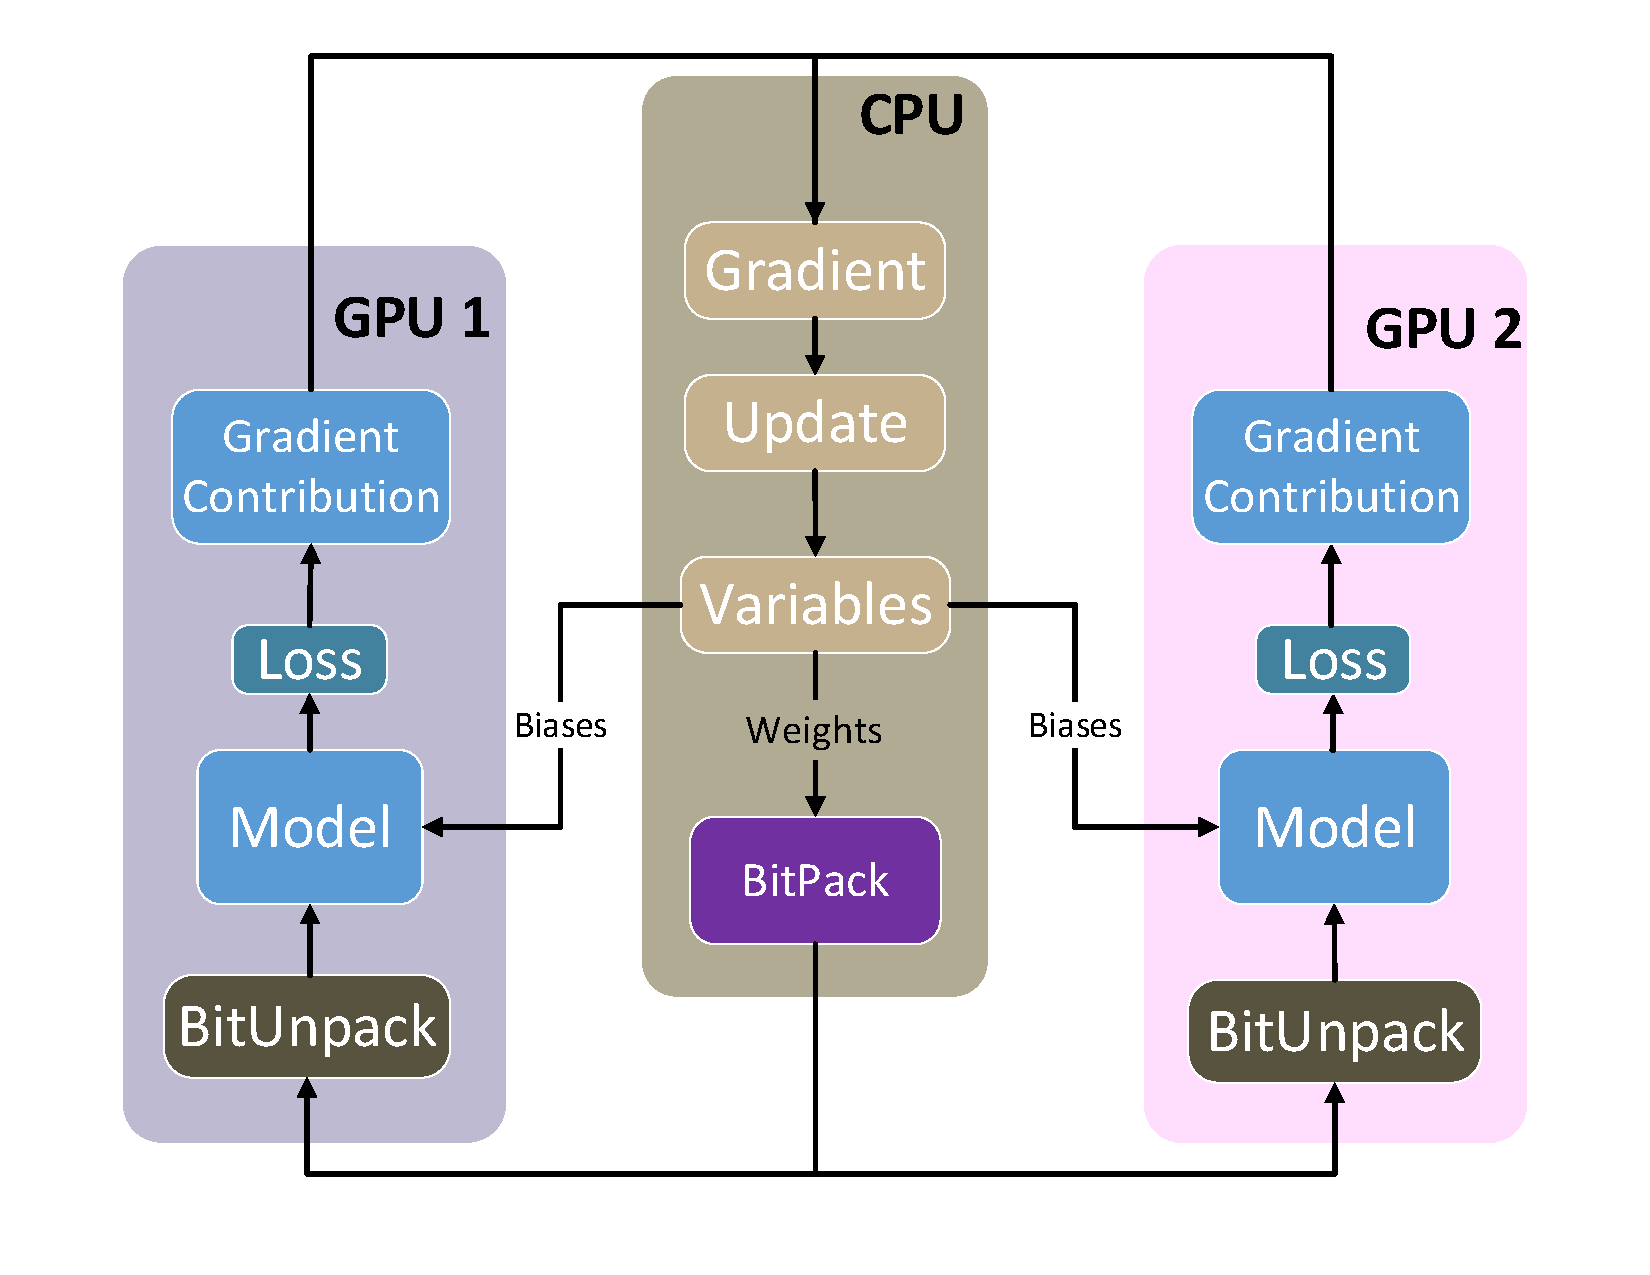
\includegraphics[scale=0.30]{figs/drawing6.pdf}}
    %\centerline{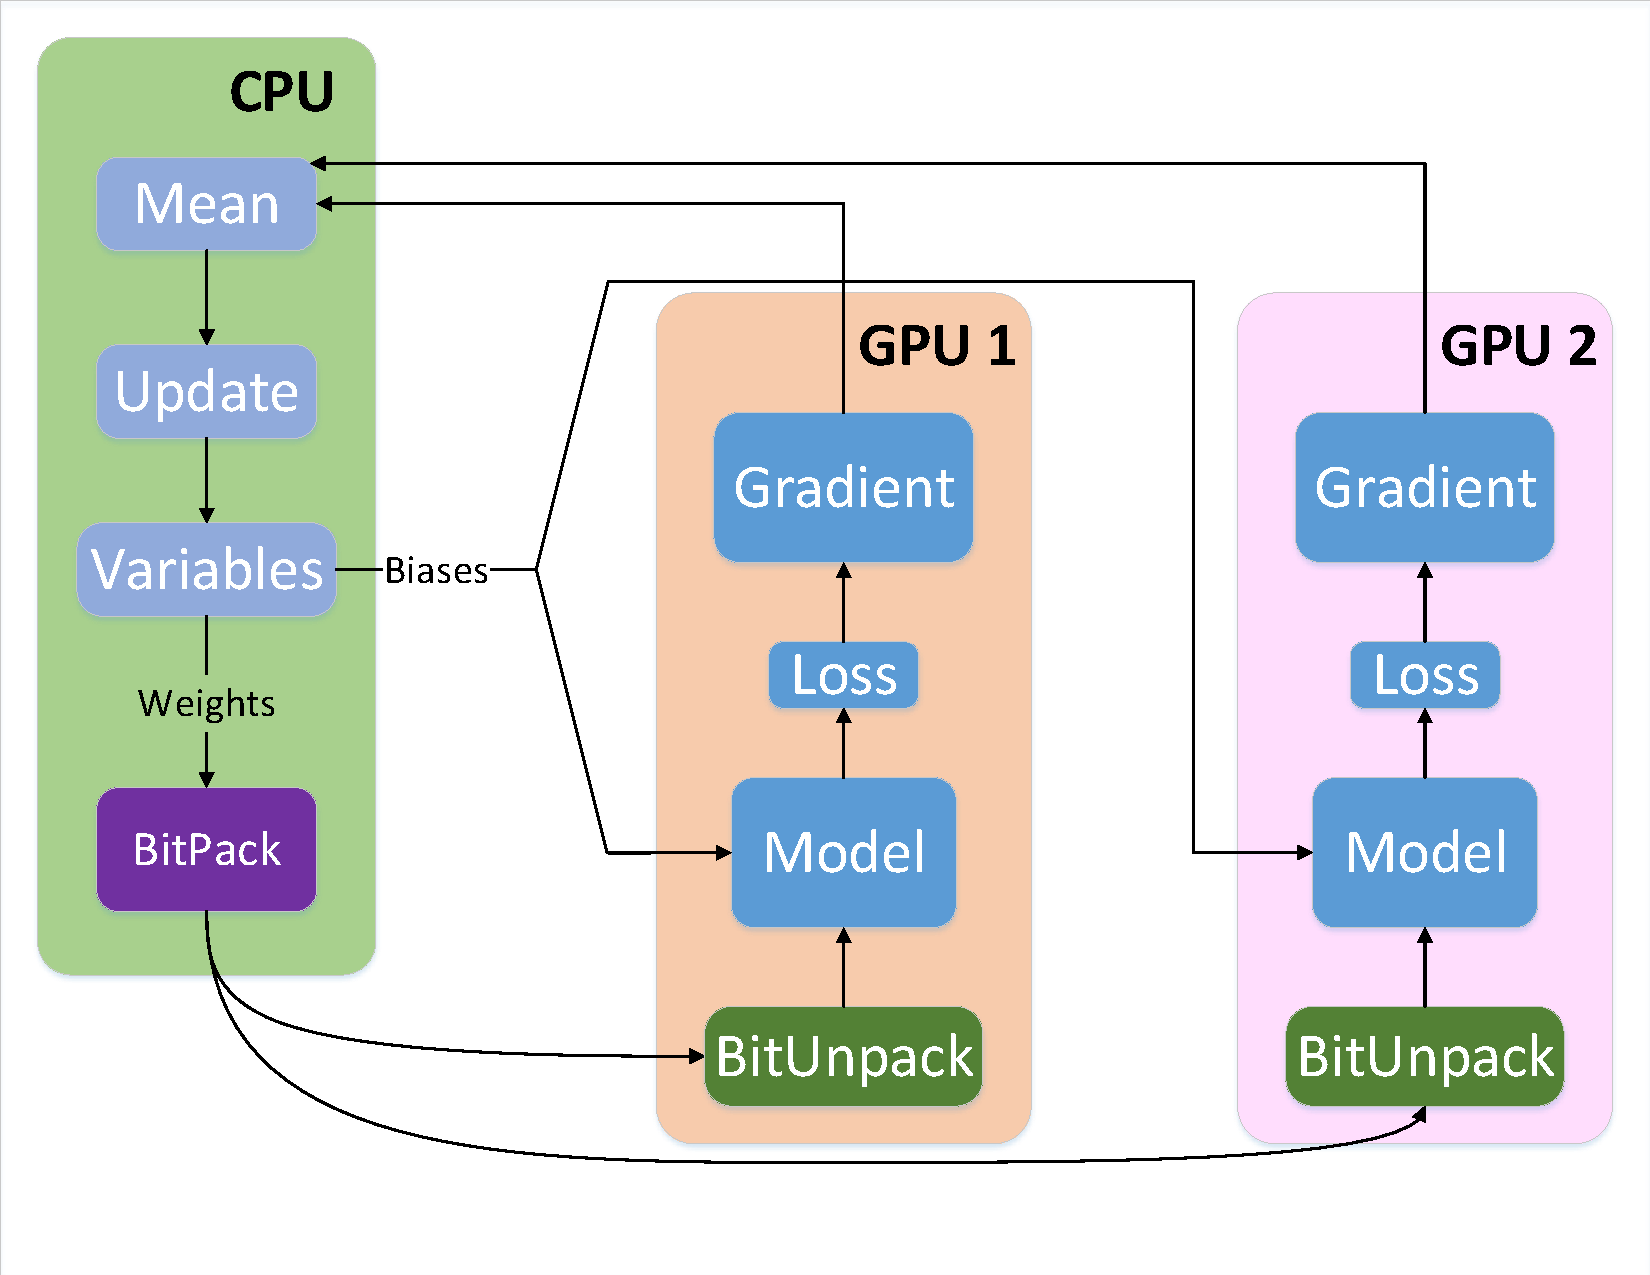
\includegraphics[scale=0.30]{figs/tensorflow_multigpu.pdf}}
        \caption{The ADt on a 2-GPU system. Variables include: weights which go through
    the ADt procedure and biases which are sent directly to the GPUs to build the
    network model together with the unpacked weights.}
        \label{bitpack_mgpu}
\end{figure}

The Bitpack operation runs on CPU multicore devices.
To boost Bitpack  
we use OpenMP~\cite{openmp} and 
Single-Instruction Multiple Data (SIMD) intrinsics.
OpenMP is used to run Bitpack on several threads.
The use of SIMD instructions allows Bitpack to operate at the SIMD register level, which
avoids incurring large performance penalties in the process of producing the reduced-size weights.
We implement two versions of Bitpack.
One version uses Intel's AVX2~\cite{avx} instruction set and the other one relies on AltiVec~\cite{Altivec}. 
Bitpack can be implemented on top of any SIMD instruction set architecture supporting simple byte shuffling instructions at the register level.
The Bitunpack procedure runs on the GPUs.

It can be trivially parallelized since each weight is mapped
to a single 32-bit FP variable, which means that GPUs can process a
large amount of weights simultaneously and efficiently build the DNN model.
In fact, Bitunpack incurs negligible overhead as Section~\ref{sec:performance} shows.

ADT manipulates the internal representation of network weights by discarding some bits.
We use the standard 32-bit IEEE-754 single-precision Floating Point format
~\cite{ieee754} (1 bit sign, 8 bits exponent and 23 bits mantissa) for all the computation routines.
The Bitpack method considers network weights as 32-bit 
words where rounding to $N$ bits means discarding the lowest $32-N$ bits.

\begin{algorithm}%[H]%algorithm* occupies full page
\caption{High Level Pseudo-code Version of Bitpack}
\label{alg:bitpack_na\"{i}ve}
{\fontsize{9}{9}\selectfont
\begin{algorithmic}[1]
    \State W
    \Comment Array of 32-bit Floating Point values containing weights
    \State Pw
    \Comment Array containing the reduced precision weights
    \State RoundTo
    \Comment Number of bytes to keep per weight
    \State POffset := 0
    \Comment Indicates the current size (in bytes) of Pw
    \For {weight \textbf{in} W}
        \State Pw[POffset : POffset+RoundTo] := weight[0 : RoundTo]
        \Comment Copy most significant RoundTo bytes to Pw
        \State POffset := POffset + RoundTo
    \EndFor
\end{algorithmic}
}
\end{algorithm}


\subsection{Bitpack}
\label{subsec:bitpack}
A high-level version of the Bitpack procedure in terms of pseudo-code is illustrated by 
Algorithm~\ref{alg:bitpack_na\"{i}ve}.
The algorithm requires a couple of arrays: the input array $W$, which contains all the weights of a certain network layer, and an 
output array $Pw$, which stores the compressed versions of these weights. 
The algorithm goes through 
the entire $W$ input array, per each weight, copies the most 
significant $RoundTo$ bytes to the output array $Pw$.
Our Bitpack implementation manipulates data at the byte granularity.
We do not observe significant performance benefits when operating at finer granularity in the experiments we run.
The AWP algorithm described in Section~\ref{sec:adaptive} determines the data representation format per each network layer.  
The number of bits of the chosen format is rounded to the nearest number of bytes
that retains all of its information (E.g., if AWP provides the value 14, $RoundTo$ will be set to 2 bytes).
The $Pw$ array is sent to the GPUs once the Bitpack procedure finishes compressing network weights.
%Currently, the host (CPU) and device (GPU) transfer byte stream so a packing
%algorithm with a granularity beyond one byte (8-bit) incurs more complexity and
%has little impact on the communication footprint. Hence, all the bitpack
%algorithm variants we are going to introduce below have a granularity of one byte.

Deep networks usually contain tens or even hundreds of millions of 
weights~\cite{alexnet, alexnet2, vgg}, which makes any trivial implementation 
of Algorithm~\ref{alg:bitpack_na\"{i}ve} not applicable in practice.
We mitigate compression costs by observing that Algorithm~\ref{alg:bitpack_na\"{i}ve} is trivially parallel since processing one weight just requires the $RoundTo$ parameter.
Algorithm~\ref{alg:bitpack_omp} shows how to parallelize the Bitpack procedure by using OpenMP threads.
Each thread takes care of a certain portion of the array storing network weights.

\begin{algorithm}%[H]%algorithm* occupies full page
\caption{Bitpack with OpenMP}
\label{alg:bitpack_omp}
{\fontsize{9}{9}\selectfont
\begin{algorithmic}[1]
    \State W 
    \Comment Array of 32-bit Floating Point values containing weights
    \State Pw
    \Comment Array containing the reduced precision weights
    \State RoundTo 
    \Comment Number of bytes to keep per weight 
    \State NumThreads
    \Comment Number of OpenMP threads
    \State \textcolor{orange} {\#pragma omp parallel for} %public(Weights, Pweights, RoundTo, workload) 
%    \Comment Distribute a portion of weights W and Pw across OpenMP processes
      \For {weight \textbf{in} W}
            \State POffset := Corresponding position in Pw
            \State Pw[POffset : POffset+RoundTo] := weight[0 : RoundTo]
            \Comment Copy the most significant RoundTo bytes to Pw
      \EndFor
\end{algorithmic}
}
\end{algorithm}

\subsection{Single Instruction Multiple Data Bitpack}
Since all weights within one layer are processed in the same way by the Bitpack procedure, we can leverage Single Instruction Multiple Data (SIMD) instructions to vectorize it.
Most state-of-the-art architectures implement SIMD instruction set: IBM's 
AltiVec~\cite{Altivec}, Intel's Advanced Vector Extensions (AVX)~\cite{avx}, and ARM's Neon~\cite{neon}.
In our experiments we use
Intel's AVX2~\cite{avx}, which implements a set of SIMD 
instructions operating over 256-bit registers, and IBM's AltiVec instruction 
set~\cite{Altivec}, which has SIMD instructions operating over 128-bit registers.
Section~\ref{sec:setup} describes the specific details of our evaluation considering both x86 and POWER architectures.
%There are also a set of intrinsic C/C++ that expose the AVX2 instructions to the software stack.  
%Intel provides a set of intrinsics for programming using the 
%SIMD instructions in C/C++, we henceforth will refer to the intrinsics rather than the 
%actual instructions.

Figure~\ref{bitpack_avx2} shows the byte-level operations of SIMD-based Bitpack applied to eight 32-bit weights and implemented with AVX2. 
The \textit{RoundTo} parameter is set to 3, which implies discarding the last 8 bits of 
each weight since the target data representation is 24-bit long. 
First, eight 32-bit Floating Point weights are loaded to a 256-bit register.
%of the 16 
%256-bit AVX2 registers. 
In the next step, we use \textit{\_mm256\_shuffle\_epi8} to shuffle the least significant
eight bits of each weight to the least significant bits of their respective 128-bit lane 
(see the grey area of Figure~\ref{bitpack_avx2} Step 2) and pack the rest of the bits 
together. 
Afterwards we use \textit{\_mm256\_permutevar8x32\_epi32} to do the same operation 
across the two 128-bit lanes. 
Finally, we use \textit{\_mm256\_maskstore\_epi32} to just store  
the resulting 192 bits to the target array.
Not all AVX2 instructions operate over the entire 256-bit register.
Instead, many of
them conceive the register as two 128-bit lanes and operate on them separately.
This is the reason way we can not carry out Steps 2 and 3 by using a single AVX2 instruction.


\definecolor{lightgray}{gray}{0.5}
\begin{figure}%[bhtp]
    \centering
    \begin{bytefield}[bitwidth=0.75em, bitformatting={\tiny},endianness=big]{32}
        \wordbox{2}{\textit{\fontsize{8}{8} \selectfont 
            Step 1: Load 8 32-bit weights into a 256-bit AVX2 register. 
            \textcolor{cyan}{(\_mm256\_loadu\_si256)}}} \\ 
        \bitboxes{4}{{\tiny $H_{3..0}$}&{\tiny $G_{3..0}$}&{\tiny $F_{3..0}$}&
                    {\tiny $E_{3..0}$}&{\tiny $D_{3..0}$}&
                    {\tiny $C_{3..0}$}&{\tiny $B_{3..0}$}&{\tiny $A_{3..0}$}} \\
        \bitheader{0,3,7,11,15,19,23,27,31} \\
        \wordbox{2}{\textit{\fontsize{8}{8} \selectfont
            Step 2: Pack weights on the 2 128-bit lanes.
            \textcolor{cyan}{(\_mm256\_shuffle\_epi8)}}} \\
        \bitboxes{3}{{\tiny $H_{3..1}$}} & 
        \bitboxes{3}{{\tiny $G_{3..1}$}} & 
        \bitboxes{3}{{\tiny $F_{3..1}$}} & 
        \bitboxes{3}{{\tiny $E_{3..1}$}} & 
        \bitbox{4}{\color{lightgray}\rule{\width}{\height}} &
        \bitboxes{3}{{\tiny $D_{3..1}$}} &
        \bitboxes{3}{{\tiny $C_{3..1}$}} &
        \bitboxes{3}{{\tiny $B_{3..1}$}} &
        \bitboxes{3}{{\tiny $A_{3..1}$}} &
        \bitbox{4}{\color{lightgray}\rule{\width}{\height}} \\
        \bitheader{0,3,6,9,12,15,19,22,25,28,31} \\
        \wordbox{2}{\textit{\fontsize{8}{8} \selectfont
            Step 3: Pack the 8 weights together by rearranging 32-bit across 
            128-lanes.
            \textcolor{cyan}{(\_mm256\_permutevar8x32\_epi32)}}} \\
        \bitboxes{3}{{\tiny $H_{3..1}$}} & 
        \bitboxes{3}{{\tiny $G_{3..1}$}} & 
        \bitboxes{3}{{\tiny $F_{3..1}$}} & 
        \bitboxes{3}{{\tiny $E_{3..1}$}} & 
        \bitboxes{3}{{\tiny $D_{3..1}$}} &
        \bitboxes{3}{{\tiny $C_{3..1}$}} &
        \bitboxes{3}{{\tiny $B_{3..1}$}} &
        \bitboxes{3}{{\tiny $A_{3..1}$}} &
        \bitbox{8}{\color{lightgray}\rule{\width}{\height}} \\
        \bitheader{0, 7, 10, 13, 16, 19, 22, 25, 28, 31} \\
        \wordbox{2}{\textit{\fontsize{8}{8} \selectfont
            Step 4: Store the most significant 24 bytes (192 bits) of data into 
            the target array. \textcolor{cyan}{(\_mm256\_maskstore\_epi32)}}} \\
    \end{bytefield}
	\vspace{-0.5cm}
	\caption{Bitpack implemented with AVX2, RoundTo=3}
	\label{bitpack_avx2}
\end{figure}

%Algorithm~\ref{alg:bitpack_omp_avx} summarizes our implementation of the Bitpack procedure with AVX2.
%It exploits two-level parallelism: first, the input array of weights is distributed across several threads.
%Second, within each thread, the compression of each eight 32-bit weights subset is performed at the register level by means of byte shuffling instructions.  
%This sophisticated procedure exploiting parallelism at both thread and SIMD register levels uses all the available hardware at the multicore level and avoids costly memory accesses.

\begin{algorithm}%[H]%algorithm* occupies full page
\caption{Bitpack with OpenMP + AVX2}
\label{alg:bitpack_omp_avx}
{\fontsize{9}{9}\selectfont
\begin{algorithmic}[1]
    \State W
    \Comment Array of 32-bit Floating Point values containing weights
    \State Pw
    \Comment Array containing the reduced precision weights
    \State RoundTo
    \Comment Number of bytes to keep per weight
    \State \textcolor{orange} {\#pragma omp parallel for} %public(Weights, Pweights, RoundTo, workload) 
%    \For {process := 0 \ldots NumProcesses}
%        \State Distribute a portion of weights W and Pw across OpenMP processes
    \For {weights \textbf{in} W}
        \State \textcolor{cyan}{\_mm256\_loadu\_si256}
        \Comment Load 8 32-bit weights 
        \State \textcolor{cyan}{\_mm256\_shuffle\_epi8}
        \Comment Compress at each 128-bit lane
        \State \textcolor{cyan}{\_mm256\_permutevar8x32\_epi32}
        \Comment Shuffle the compressed weights into the most significant bits
        \State \textcolor{cyan}{\_mm256\_maskstore\_epi32}
        \Comment Store compressed weights to the target array
    \EndFor
\end{algorithmic}
}
\end{algorithm}

\begin{algorithm}%[H]%algorithm* occupies full page
\caption{Bitunpack on GPU}
\label{alg:bitunpack}
{\fontsize{9}{9}\selectfont
\begin{algorithmic}[1]
    \State Pw
    \Comment Array containing compressed weights
    \State W
    \Comment Array of 32-bit Floating Point values containing weights
    \State RoundTo
    \Comment The number of bytes that are going to be kept
    \For{UnitId := 0 \ldots NumUnit}
    \State Distribute W and Pw across all the computation units in the GPU
        \State POffset := 0
        \For{weight in W}
            \State weight := Pw[POffset : POffset+RoundTo] $\ll$ (4 - RoundTo) * 8
            \State POffset := POffset + RoundTo
        \EndFor
    \EndFor
\end{algorithmic}
}
\end{algorithm}

Algorithm~\ref{alg:bitpack_omp_avx} summarizes our implementation of the Bitpack procedure with AVX2.
It exploits two-level parallelism: first, the input array of weights is distributed across several threads.
Second, within each thread, the compression of each eight 32-bit weights subset is performed at the register level by means of byte shuffling instructions.
This sophisticated procedure exploiting parallelism at both thread and SIMD register levels uses all the available hardware and avoids costly memory accesses.

\subsection{Bitunpack}
Once data in reduced-size format reaches the target GPU, the Bitunpack procedure immediately 
restores them into their original IEEE-754 32-bit Floating Point format. 
We display pseudo-code describing this process in Algorithm~\ref{alg:bitunpack}.
Bitunpack reads the reduced-sized weights from array $Pw$ and assigns additional bits to them. 
Bitunpack gives zero values to these additional bits.
We distribute the Bitunpack process across the whole GPU, which enables an extremely parallel scheme exploiting GPUs manycore architecture. 

The Bitunpack routine is developed using CUDA~\cite{cuda}. 
Our code  
runs in parallel on $N$ CUDA threads and the CUDA runtime handles the dynamic mapping between threads and the underlying GPU compute units.
Since each thread involved in the parallel run targets a different portion of the $Pw$ array, our Bitunpack procedure exposes a large amount of parallelism able to exploit the large number of compute units integrated into high-end GPU devices.


\section{Experimental Setup}
\label{sec:setup}

The experimental setup considers a large image dataset, three state-of-the-art neural network models and two high-end platforms.
The following sections describe all theses elements in detail.

\subsection{Image Dataset}
We consider the ImageNet ILSVRC-2012 
dataset~\cite{imagenet}.
The original ImageNet dataset includes three sets of images of 1000 classes each:
training set (1.3 million images), validation set (50,000 images) and
testing set (100,000 images).
Considering 1000 classes makes the training process around 170 hours long, which is prohibitively expensive for large experimental campaign considering different network models, batch sizes and hardware platforms.
To reduce the execution time of our experiments we consider a subset of 200 
classes for both the training and the validation dataset, which keeps the training time under manageable margins.
%  To speedup our experiments without hampering
%the quality of the results, we select a same set of 200 classes for both the
%training set and the validation set as our dataset.
%For the rest of this paper, 
We refer to the 200 and 1000 classes datasets as ImageNet200 and ImageNet1000, respectively.
Since it is a common practice~\cite{vgg}, we evaluate the ability of a certain network in 
properly dealing with the ImageNet ILSVRC-2012 dataset in terms of the top-5 validation error computed over the validation set.

\subsection{DNN Models and Training Parameters}
We apply the AWP algorithm along with the ADT procedure on three state-of-the-art 
DNN models: a modified version of Alexnet~\cite{alexnet} with an extra fully-connected layer of size 4096, the configuration A of the VGG model~\cite{vgg} and the Resnet network~\cite{resnet}. 
All hidden layers are equipped with a Rectified Linear Units (ReLU)~\cite{alexnet}.
The exact configurations of the three neural networks are shown in Table~\ref{table:config}. 
The Alexnet model is composed of 5 convolutional layers and 4 fully-connected ones, VGG contains 8 convolutional layers and 3 fully-connected ones and Resnet is composed of 33 convolutional layers and a single fully-connected one.

% Please add the following required packages to your document preamble:
% \usepackage{multirow}
\begin{table}[]
\caption{Neural network configurations: The convolutional layer parameters are denoted 
as ``conv<receptive field size>-<number of channels>''. The ReLU activation 
    function is not shown for brevity. The building blocks of Resnet
    and the number of times they are applied are shown in a single cell.}
    \begin{tabular}{|P{2.5cm}|P{2.5cm}|P{2.5cm}|}
\hline
    \textbf{Alexnet} & \textbf{VGG}  & \textbf{Resnet-34}  \\ \hline
\multicolumn{3}{|c|}{input(224x224 RGB image)}                                                                                                                                                 \\ \hline
conv11-64                                                  & conv3-64                                                      & conv7-64                                                           \\ \hline
\multicolumn{3}{|c|}{maxpool}                                                                                                                                                                  \\ \hline
conv5-192                                                 & conv3-128                                                     & \begin{tabular}[c]{@{}c@{}}conv3-64\\ conv3-64\\ x3\end{tabular}   \\ \hline
\multicolumn{2}{|c|}{maxpool}                                                                                             &                                                                    \\ \hline
conv3-384                                                 & \begin{tabular}[c]{@{}c@{}}conv3-256\\ conv3-256\end{tabular} & \begin{tabular}[c]{@{}c@{}}conv3-128\\ conv3-128\\ x4\end{tabular} \\ \hline
\multicolumn{2}{|c|}{maxpool}                                                                                             &                                                                    \\ \hline
conv3-384                                                  & \begin{tabular}[c]{@{}c@{}}conv3-512\\ conv3-512\end{tabular} & \begin{tabular}[c]{@{}c@{}}conv3-256\\ conv3-256\\ x6\end{tabular} \\ \hline
\multicolumn{2}{|c|}{maxpool}                                                                                             &                                                                    \\ \hline
conv3-256                                                 & \begin{tabular}[c]{@{}c@{}}conv3-512\\ conv3-512\end{tabular} & \begin{tabular}[c]{@{}c@{}}conv3-512\\ conv3-512\\ x3\end{tabular} \\ \hline
\multicolumn{2}{|c|}{maxpool}                                                                                             & avgpool                                                            \\ \hline
\multicolumn{2}{|c|}{FC-4096}                                                                                             & \multicolumn{1}{l|}{\multirow{2}{*}{}}                             \\ \cline{1-2}
\begin{tabular}[c]{@{}c@{}}FC-4096\\ FC-4096\end{tabular} & \multicolumn{1}{c|}{FC-4096}                                  & \multicolumn{1}{l|}{}                                              \\ \hline
\multicolumn{3}{|c|}{FC-200}                                                                                                                                                                   \\ \hline
\multicolumn{3}{|c|}{softmax}                                                                                                                                                                  \\ \hline
\end{tabular}
\label{table:config}
\end{table}

%\begin{table}
%\caption{Neural network configurations: The convolutional layer parameters are denoted 
%as ``conv<receptive field size>-<number of channels>''. The ReLU activation 
%function is not shown for brevity.}
%%\fontsize{3}{3}\selectfont
%%\resizebox{.45\textwidth}{!}{
%\end{tabular}
%%}
%%\vspace{0.2cm}
%\label{table:config}
%%\vspace{-0.5cm}
%\end{table}


We use momentum SGD~\cite{momentum} to guide the training process with 
momentum set to 0.9. 
The training process is regularized by weight decay and  the $L_{2}$ 
penalty multiplier is set to $5\times10^{-4}$. 
We apply a dropout 
regularization value of 0.5 to fully-connected layers.
We initialize the weights using a zero-mean normal distribution 
with variance $10^{-2}$. 
The biases are initialized to $0.1$ for Alexnet and $0$ for both VGG and Resnet networks.
For the Alexnet and VGG models we consider training batch sizes of 64, 32 and 16.
To train the largest network we consider, Resnet, we consider batch sizes of 128, 64 and 32.
The 16 batch size incurs in a prohibitively expensive training process for Resnet and, therefore, we do not use it in our experimental campaign. 
%
%There are several factors to take into consideration that affect the
%benefits provided by this papers' proposals.
%Among the most important ones we have the number of weights of the considered neural network, 
%which define the size of the data transfers over which our solution is deployed, 
%or the batch size, which defines the number of samples each batch is composed of. 
%Since the network weights are updated every time a batch is processed, the smaller 
%the batch size is, the more frequent are the weight updates and, thus, the larger 
%is the potential of our solution for improving performance.
%In order to cover these factors,
%we train both neural networks using a set of three batch sizes: 64, 32 and 16.
%

For Alexnet we set the initial learning rate to $10^{-2}$ for the 64 batch size and decrease it by factors of 2 and 4 for the 32 and 16 batch sizes, respectively.
In the case of VGG we 
set the initial learning rate to $10^{-2}$ for the 64, 32 and 16 batch sizes, as in the state-of-the-art~\cite{vgg}.  
In the case of Resnet the learning rate is $10^{-2}$ for the 
batch size of 32 and 0.1 for the rest. 
For all network models we apply exponential decay to the learning rate throughout the whole training process in a way the learning rate decays every 30 batches by a factor of 0.16, as previous work suggests~\cite{alexnet2}.
For Resnet we obtain better results by adapting precision at the Resnet building blocks level~\cite{resnet} instead of doing so in a per-layer basis.
%\textcolor{cyan}{Our preliminary experiments suggest that by applying our approach 
%to all of the layers separately on Resnet does not provide any benefit. Instead, 
%we group the layer in terms of the resnet building blocks~\cite{resnet} and apply our approach on 
%that level.}

\subsection{Implementation}
Our code is written in Python on top of Google Tensorflow~\cite{tensorflow}.
Tensorflow is a data-flow and graph-based numerical library where 
the actual computation is carried out according to a computational graph 
constructed beforehand.
The computational graph defines the order and the type of computations that are 
going to take place. It supports NVIDIA's NCCL library.

To enable the use of both Bitpack and Bitunpack routines, we integrate them into Tensorflow using its C++ API.
Tensorflow executes the two routines before sending 
the weights from the CPU to the GPU and right after receiving the weights on the 
GPU side, respectively.
The Bitpack routine is implemented using the OpenMP 4.0 programming model. 
There are two versions of this routine using either Intel's AVX2 or AltiVec instructions, as explained in Section~\ref{sec:approx}.
Bitunpack is implemented using CUDA 8.0 and CUDA 10.0 respectively on the two 
platforms~\cite{cuda}.

\subsection{Hardware Platforms}
\label{sec:platform}
We conduct our experiments on two clusters featuring the x86 and POWER architectures.
The x86 machine is composed of two 8-core Intel Xeon
\textregistered E5-2630 v3 (Haswell) at 2.4 GHz and a 20 MB L3 shared cache memory each. 
It is also equipped with two Nvidia Tesla K80 accelerators, each of which hosts two 
Tesla GK210 GPUs.
It has 128 GB of main memory, distributed in 8 DIMMs of 16 GB DDR4 @ 2133 MHz.
The 16-core CPU and the four GPUs are connected via a PCIe 3.0 x8 8GT/s.
The operating system is RedHat Linux 6.7.
Overall, the peak performance of the two 8-core sockets plus the four Tesla GK210 GPUs is 6.44 TFlop/s.

The POWER machine is composed of two 20-core IBM POWER9 8335-GTG at 3.00 GHz.  
It contains four NVIDIA Volta V100 GPUs. 
Each node has 512 GB of main memory, distributed in 16 DIMMS of 32 GB @ 2666 MHz.
The GPUs are connected to the CPU devices via a NVIDIA NVLink 2.0 interconnection~\cite{nvlink}.
The operating system is RedHat Linux 7.4.
The peak performance of the two 20-core sockets plus the four V100 GPUs is 28.85 TFlop/s.

%\begin{figure*}[!bhtp]
%        \centerline{
%            \includegraphics[scale=0.24]{figs/alex/small_3/alexnet_validation_top5_32-$A^2$DtWp.pdf}
%            \includegraphics[scale=0.24]{figs/alex/small_3/alexnet_validation_top5_16-$A^2$DtWp.pdf}
%            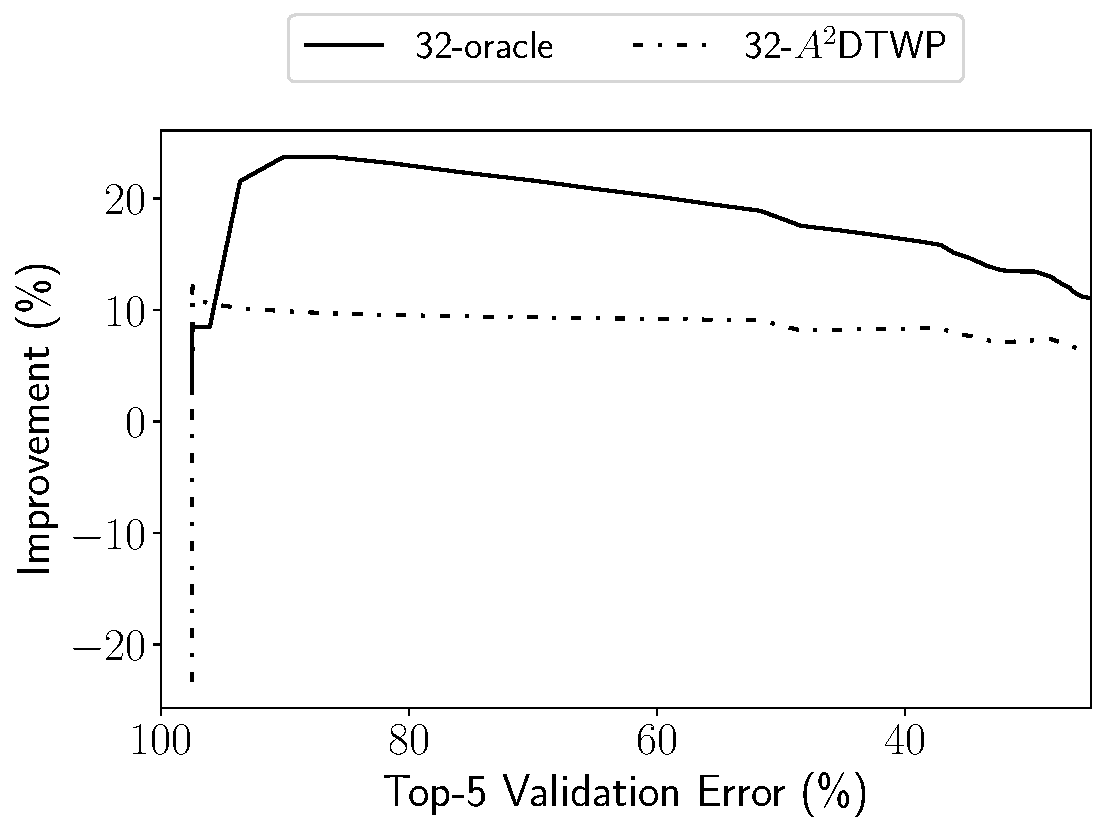
\includegraphics[scale=0.24]{figs/alex/small_3/alexnet_train_improvement_agg_top5_32-baseline.pdf}
%            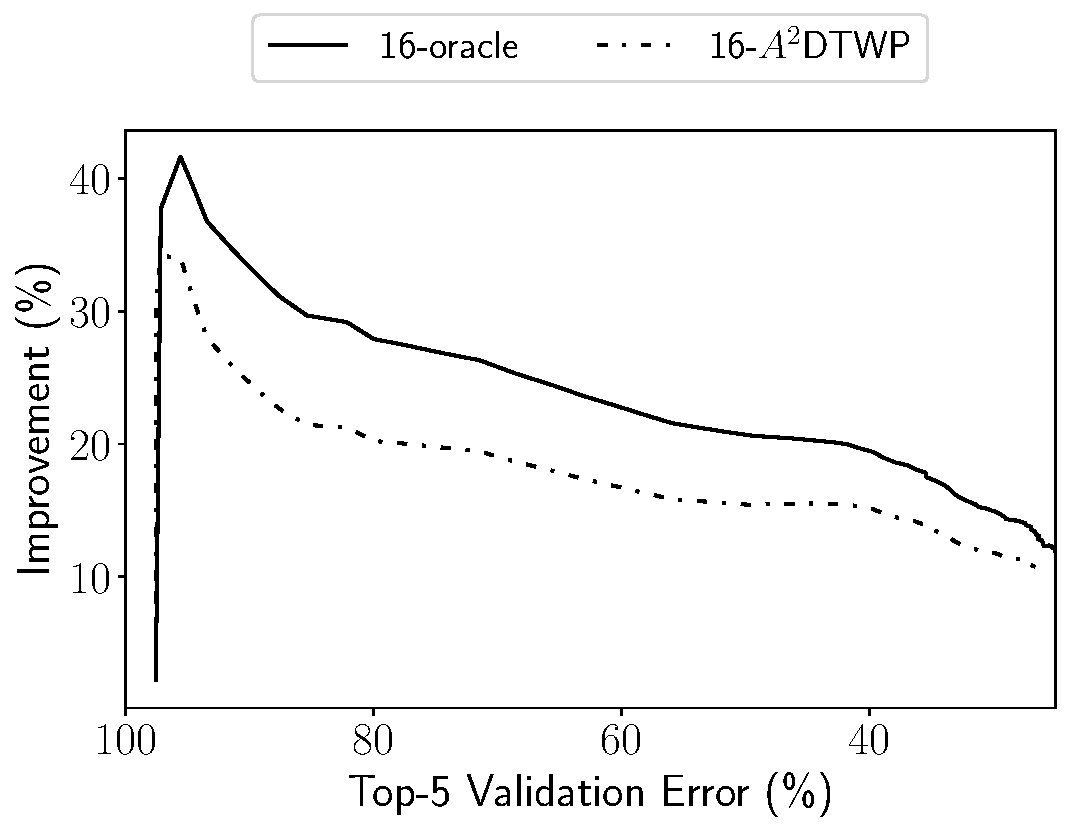
\includegraphics[scale=0.24]{figs/alex/small_3/alexnet_train_improvement_agg_top5_16-baseline.pdf}
%        }
%    \vspace{-0.4cm}
%    \caption{Results on Alexnet with two batch sizes: 32 and 16. The left
%    two figures show the top-5 validation error evolution of
%    \textit{baseline}, \textit{oracle} and \textit{$A^2$DTWP}.
%    The right two figures provide information on the performance improvement of
%    \textit{oracle} and \textit{$A^2$DTWP} against \textit{baseline}
%    during the training process. Experiments run on the x86 system.
%    \vspace{-0.5cm}
%    }
%        \label{alex_improv}
%\end{figure*}

\begin{figure*}[!bhtp]
    \hbox{%\hspace{7.0mm}
        \centerline{
            \includegraphics[scale=0.450]{figs/alex/small_3/alexnet_validation_top5_32-$A^2$DtWp.pdf}
            \includegraphics[scale=0.450]{figs/alex/small_3/alexnet_validation_top5_16-$A^2$DtWp.pdf}
        }
    }
    \hbox{%\hspace{7.0mm}
        \centerline{
            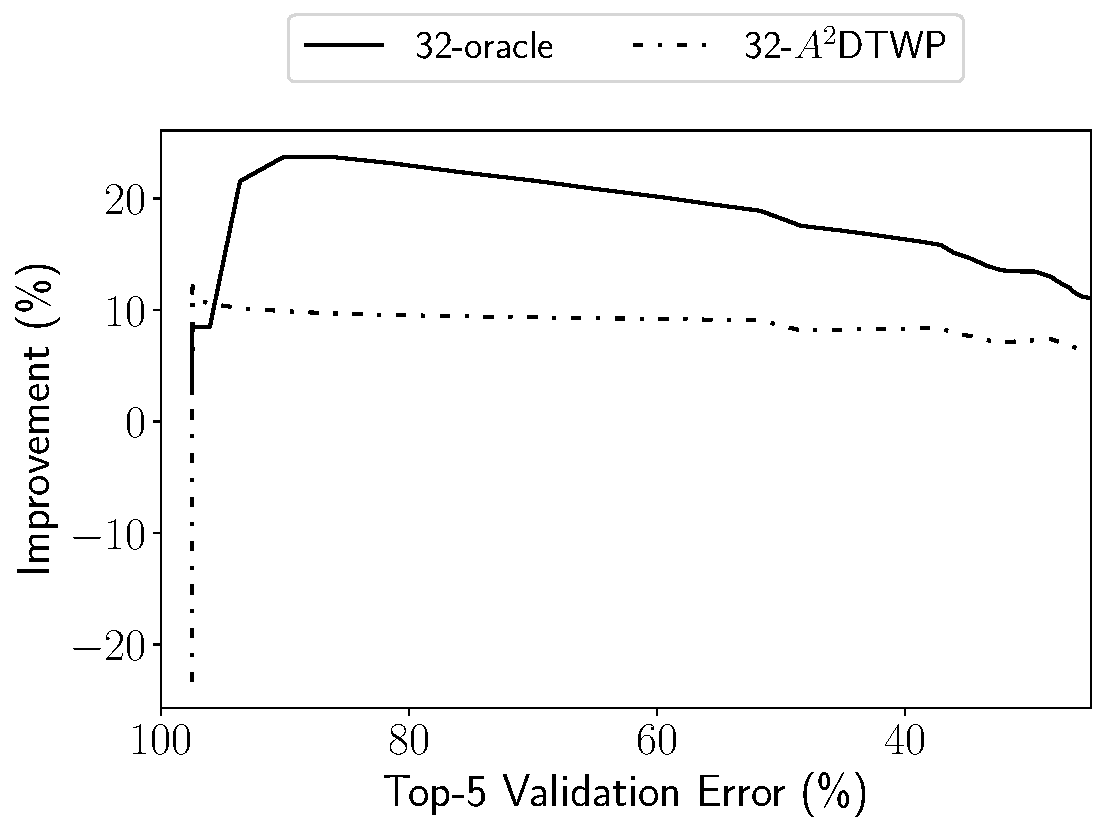
\includegraphics[scale=0.450]{figs/alex/small_3/alexnet_train_improvement_agg_top5_32-baseline.pdf}
            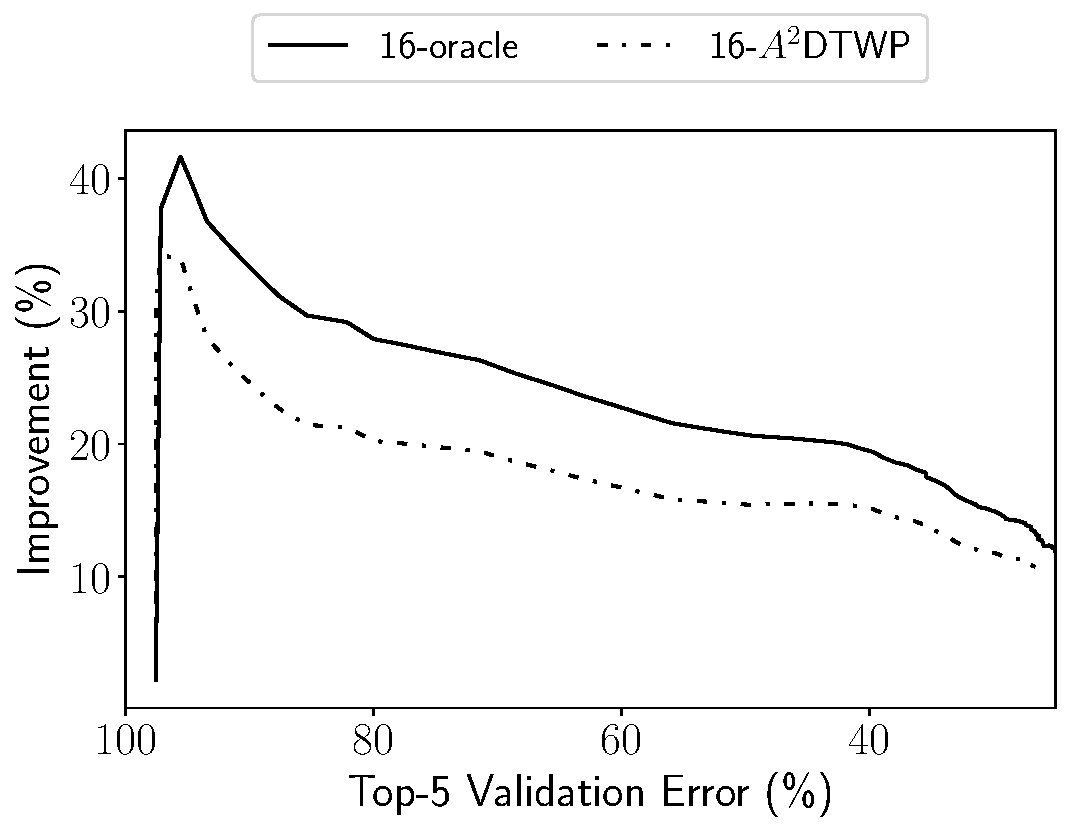
\includegraphics[scale=0.450]{figs/alex/small_3/alexnet_train_improvement_agg_top5_16-baseline.pdf}
        }
    }
    \caption{Alexnet training considering 32 and 16 batch sizes. The 
    two upper plots show the top-5 validation error evolution of
    \textit{baseline}, \textit{oracle} and \textit{$A^2$DTWP}.
    The two bottom plots provide information on the performance improvement of
    \textit{oracle} and \textit{$A^2$DTWP} against \textit{baseline}
    during the training process. Experiments run on the x86 system.
    %\vspace{-0.5cm}
    }
        \label{alex_improv}
\end{figure*}



\section{Evaluation}
\label{sec:evalutation}
In this section we evaluate the capacity of the AWP algorithm and the ADT procedure to accelerate DNNs training. 
We show how our proposals are able to accelerate the training phase of relevant DNN models without reducing the accuracy of the network. 
%to classify large image data sets. 

\subsection{Methodology}
\label{sec:evaluation1}

%\begin{figure*}[!bhtp]
%    \vspace{0.1cm}
%    \centerline{
%        \includegraphics[scale=0.24]{figs/vgg/small_3/vgg_validation_top5_64-$A^2$DtWp.pdf}
%        \includegraphics[scale=0.24]{figs/vgg/small_3/vgg_validation_top5_32-$A^2$DtWp.pdf}
%        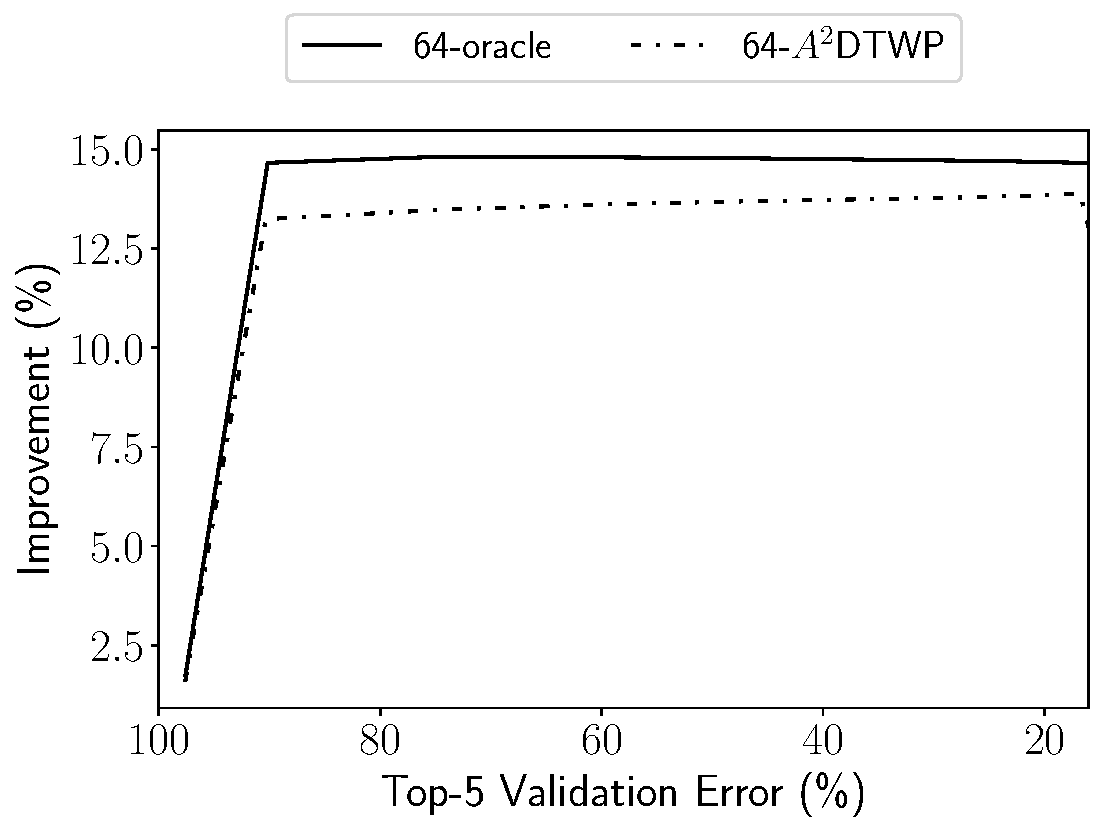
\includegraphics[scale=0.24]{figs/vgg/small_3/vgg_train_improvement_agg_top5_64-baseline.pdf}
%        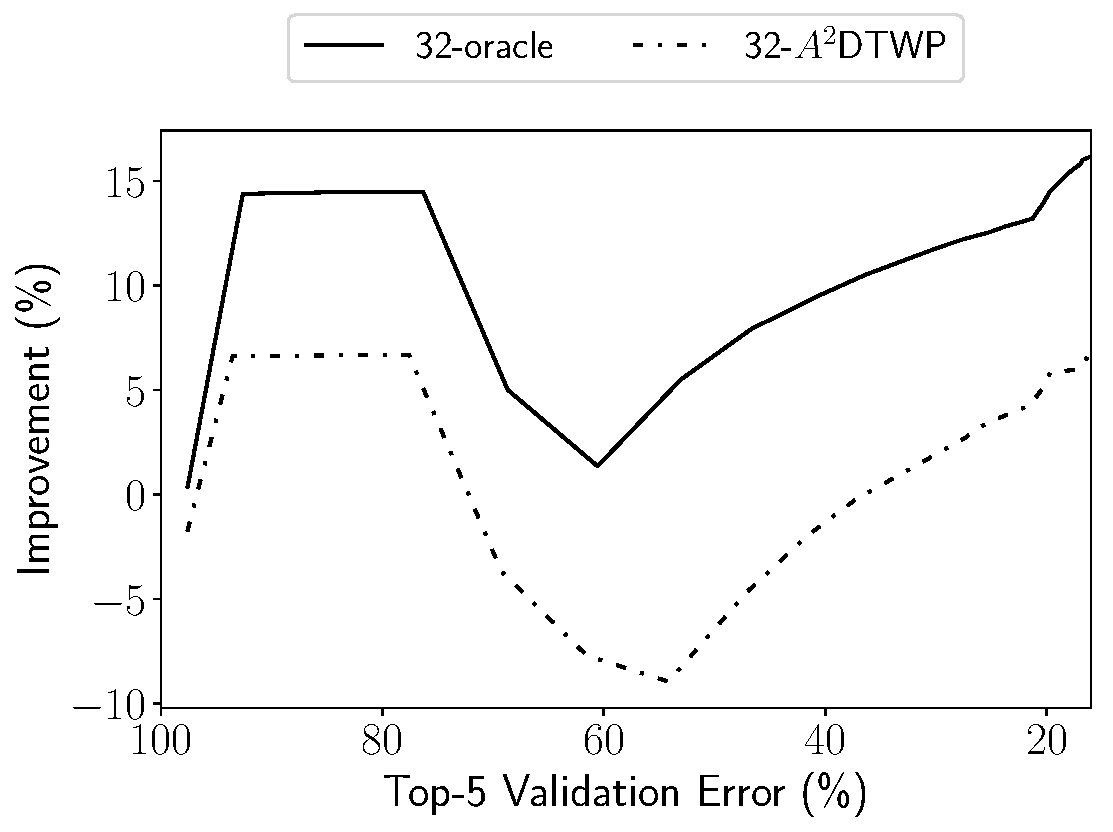
\includegraphics[scale=0.24]{figs/vgg/small_3/vgg_train_improvement_agg_top5_32-baseline.pdf}
%    }
%    \vspace{-0.4cm}
%    \caption{Results on VGG with two batch sizes: 64 and 32. The left
%    two figures show the top-5 validation error evolution of
%    \textit{baseline}, \textit{oracle} and \textit{$A^2$DTWP}.
%    The right two figures provide information on the performance improvement of
%    \textit{oracle} and \textit{$A^2$DTWP} against \textit{baseline} during the
%    training process. Experiments run on the x86 system.
%    %\rephrased{Figures upgraded from using continuous lines to using points}
%    }
%        \label{vgg_improv}
%    %\vspace{-0.5cm}
%\end{figure*}

\begin{figure*}[!bhtp]
    \hbox{%\hspace{7.0mm}
        \centerline{
            \includegraphics[scale=0.450]{figs/vgg/small_3/vgg_validation_top5_64-$A^2$DtWp.pdf}
            \includegraphics[scale=0.450]{figs/vgg/small_3/vgg_validation_top5_32-$A^2$DtWp.pdf}
        }
    }
    \hbox{%\hspace{7.0mm}
        \centerline{
            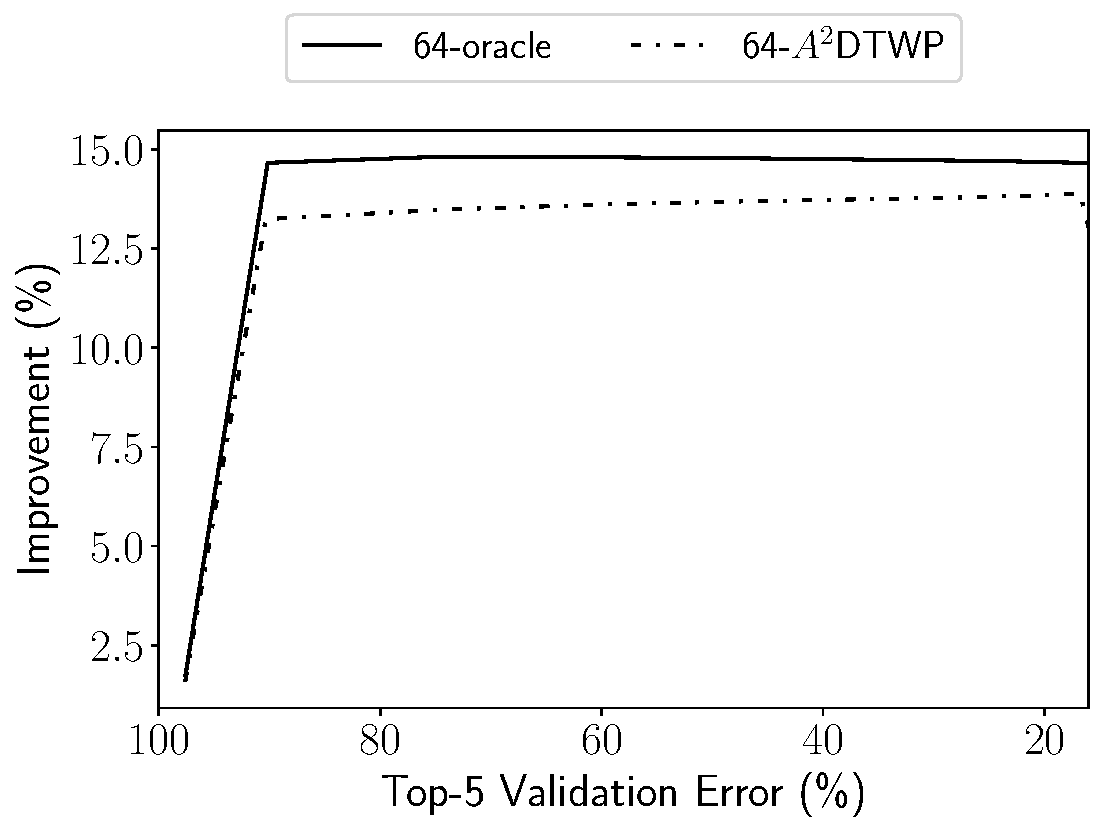
\includegraphics[scale=0.450]{figs/vgg/small_3/vgg_train_improvement_agg_top5_64-baseline.pdf}
            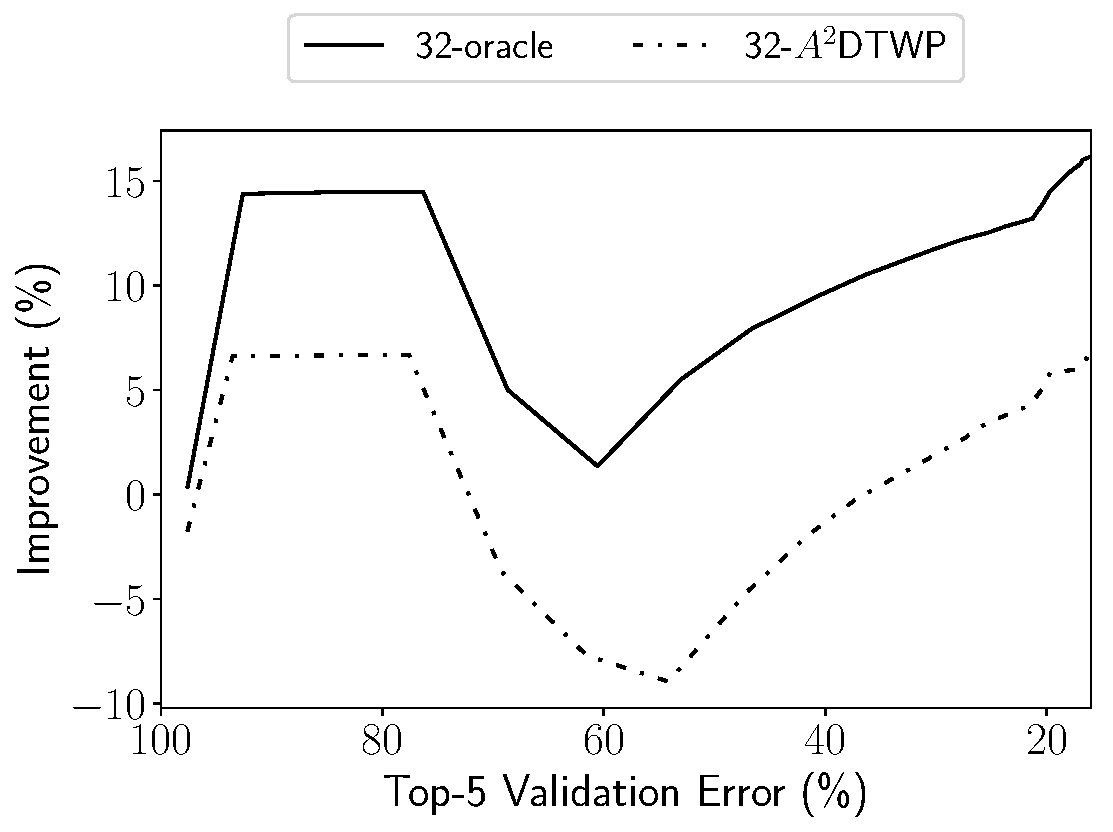
\includegraphics[scale=0.450]{figs/vgg/small_3/vgg_train_improvement_agg_top5_32-baseline.pdf}
        }
    }
    \caption{VGG training considering 64 and 32 batch sizes. The 
    two upper plots show the top-5 validation error evolution of
    \textit{baseline}, \textit{oracle} and \textit{$A^2$DTWP}.
    The two bottom figures provide information on the performance improvement of
    \textit{oracle} and \textit{$A^2$DTWP} against \textit{baseline} during the
    training process. Experiments run on the x86 system.
    %\rephrased{Figures upgraded from using continuous lines to using points}
    }
    \label{vgg_improv}
    %\vspace{-0.5cm}
\end{figure*}

%We conduct a set of experiments on several batch sizes (16, 32, 64) for both Alexnet and VGG. 
Our experimental campaign considers batch sizes of 64, 32 and 16 for the Alexnet and VGG models and 128, 64 and 32 for the Resnet network.
For each model and batch size, the \emph{baseline} run uses the 32-bit Floating Point precision for the whole training. 
The data represention formats we consider to transfer weights from the CPU to the GPU are:
8-bit (1 bit for sign, 7 bits for exponent), 16-bit (1 bit for sign, 8 for exponent, 7 for mantissa), 24-bit (1 bit for sign, 8-bits for exponent and 15 bits for mantissa) and 32-bits (1 bit for sign, 8 bits for exponent and 23 bits for mantissa).
We train the network models with dynamic data representation by applying the AWP algorithm along with the ADT procedure.
We denote this approach combining ADT and AWP as \textit{$A^2$DTWP}.  
For each DNN and batch size, we select the data representation format that first 
reaches the 35\%, 25\% and 15\% accuracy thresholds for Resnet, Alexnet and VGG, respectively, and we 
denote this approach as \emph{oracle}.
For the case of the \emph{oracle} approach, data compression is done via ADT.
The closer \textit{$A^2$DTWP} is to \emph{oracle}, the better is the AWP algorithm in identifying the best data representation format.

During training we sample data in terms of elapse time and validation error every 4000 batches. 
The total number of training batches corresponding to the whole ImageNet200 dataset are 16020, 8010, 4005 and 2002 for batch sizes 16, 32, 64 and 128, respectively.
The values of $AWP$ parameters $T$, $INTERVAL$, and $N$ are determined in the following way:
In the case of $T$ we monitor the execution of several epochs until we observe a drop in the validation error. 
We then measure the average change, considering all layers, of weights' $l^2$-norm during this short monitoring period.
The obtained values of $T$ are $-5\times10^{-2}$, $-2\times10^{-3}$ and $-2\times10^{-5}$ for Alexnet, VGG and Resnet, respectively.
We set the $INTERVAL$ parameter to $4000$ for both AlexNet and VGG and $2000$ for Resnet. 
These values correspond to a single batch (for the ImageNet200 dataset and batch sizes 64 and 128) and avoid premature precision switching due to numerical fluctuations.  
We set $N$ to $8$ since the smallest granularity of our approach is 1 byte.
AWP initially applies 8-bit precision to all layers.
We use ImageNet200 in Sections~\ref{sec:alexnet}, ~\ref{sec:VGG}, ~\ref{sec:Resnet}, ~\ref{sec:Average}, and ~\ref{sec:performance}.
Section~\ref{sec:ImageNet1000} uses ImageNet1000.

\subsection{Evaluation on Alexnet}
\label{sec:alexnet}
The evaluation considering the Alexnet model on the x86 system is shown in  
Figure~\ref{alex_improv}, which plots detailed results considering batch sizes of 
32 and 16, and Figure~\ref{fig:all}, which shows the total execution time of the 
\textit{oracle} and \textit{$A^2$DTWP} policies normalized to the \textit{baseline} 
for the 64, 32 and 16 batch sizes on both the x86 and the POWER systems.
The two top plots of Figure~\ref{alex_improv} depict how the validation error of the 
\textit{baseline}, \textit{oracle}, and \textit{$A^2$DTWP} policies evolves 
over time for the 32 and the 16 batch sizes until the 25\% accuracy is reached.
The two bottom plots provide information regarding the performance 
improvement of both \textit{oracle} and \textit{$A^2$DTWP} over the 
32-bit \textit{baseline} with regard to a certain validation error. 
Such performance improvement is computed by looking at the time required by the 
\textit{oracle} and \textit{$A^2$DTWP} techniques to reach a certain validation error with respect to the \textit{baseline}.

It can be observed in the upper left-hand side plot of Figure~\ref{alex_improv} how 
the \textit{oracle} and the \textit{$A^2$DTWP} approaches are 10.82\% and 6.61\% faster than the baseline, respectively, to reach the 25\% top-5 validation error when using a 32 batch size.
The upper right-hand side plot shows results considering a 16 batch size. 
The improvements achieved by the 
\textit{oracle} and \textit{$A^2$DTWP} approaches are 11.52\% and 10.66\%, respectively.
This demonstrates 
the efficiency of the ADT procedure in compressing and decompressing the network weights without undermining the performance benefits obtained from sending less data
from the CPU device to the GPU.
It also demonstrates the capacity of AWP to quickly identify the best data representation format per layer.

The two bottom plots of Figure~\ref{alex_improv} provide information on 
performance improvement of \textit{oracle} and \textit{$A^2$DTWP} over the \textit{baseline} during the training process.
%One of the right-hand side plots of Figure~\ref{alex_improv} shows results when considering the 32 batch size.
For the 32 batch size, \textit{oracle} reaches a peak improvement of 24.11\% when the 90\%  
validation error is reached and steadily declines from that point although it keeps a significant 
improvement of 10.82\% over the \textit{baseline} once the 25\% top-5 validation error is reached. 
\textit{$A^2$DTWP} falls in-between the \textit{baseline} and the \textit{oracle}  
and keeps its improvement above 7.03\% until it reaches the 27\% top-5 validation error.
Once it reaches the 25\% validation error \textit{$A^2$DTWP} is 6.51\% faster than the \textit{baseline}.
In conclusion, the \textit{$A^2$DTWP} policy is able to provide performance 
improvements that are close to the ones achieved by the best possible accuracy.
%while the \textit{best} reaches 9.39\% at 25\% validation error.
For the 16 batch size, the performance benefits of the 
\textit{oracle} policy reach a 41.64\% peak at the 94\% validation error point.
The \textit{$A^2$DTWP} policy reaches its maximum performance benefit, 34.21\%, when the validation error is 97\%.
At the 25\% validation error point, the \textit{oracle} and the 
\textit{$A^2$DTWP} policies reach 13.00\% and 10.75\% performance improvement, respectively.
Overall, results considering the Alexnet network for batch sizes 
32 and 16 confirm that \textit{$A^2$DTWP}, which combines both the 
AWP algorithm and the ADT procedure, successfully delivers very similar 
performance benefits to the best possible accuracy.

Figure~\ref{fig:all} shows the normalized execution time of the \textit{oracle} 
and \textit{$A^2$DTWP} policies with respect to the 32-bit FP \textit{baseline} on the x86 and the POWER systems. 
The top chart reports performance improvements of 10.75\%, 6.51\%, and 0.59\% for batch sizes 16, 32 and 64 in
the case of Alexnet runnig on the x86 system.  
For the 64 batch size, the marginal gains of \textit{$A^2$DTWP} over the \textit{baseline} are due the poor performance of the 8-bits format employed by \textit{$A^2$DTWP} at the beginning of the training process.
This format does not contribute to reduce the validation error for the 64 batch case, which makes the \textit{$A^2$DTWP} policy to fall behind the \textit{baseline} at the very beginning of the training process.  
Although \textit{$A^2$DTWP} eventually increases its accuracy and surpases the \textit{baseline}, it does not provide the same significant performance gains for Alexnet as the ones observed for batch sizes 16 and 32.

\textit{$A^2$DTWP} performance improvements on the POWER system in the case of 
Alexnet are 18.61\%, 14.25\% and 10.01\% with respect to the \textit{baseline} for batch sizes 16, 32 and 64, respectively.  
The POWER system achieves larger performance improvements than x86 since the 
Bitpack procedure can be further parallelized over the 40 cores of the POWER9 
multicore chips than the 16 cores available in the Haswell multicore devices of the x86 system. 
This mitigates the costs of weigths' compression and thus provides larger performance improvements. 

\subsection{Evaluation on VGG}
\label{sec:VGG}

Figure~\ref{vgg_improv} shows results for batch sizes 64 and 32 when using the 
VGG architecture on the x86 system. 
The upper figures display the temporal evolution of the validation error until the 15\% top-5 validation error is reached.
Like in Alexnet, both the \textit{$A^2$DTWP} and the \textit{oracle} policies outperform the \textit{baseline}.
In the case of batch size 64, both \textit{oracle} and \textit{$A^2$DTWP} 
display a similar evolution in terms of validation error, which translates to 
very close performance improvement over the baseline. 
They maintain an overall improvement of over 13.00\% against the \textit{baseline} 
during most of their training. The \textit{$A^2$DTWP} technique outperforms the baseline by 
12.88\% when reaches 15\% of top-5 validation error while the 
\textit{oracle} policy achieves the same improvement.
For batch size 32 the final improvement achieved by \textit{$A^2$DTWP} over the baseline is 5.02\%.
This improvement is not as large as the one achived for the 64 batch size since the AWP algorithm does not identify a numerical precision able to beat the \textit{baseline} until the 57\% validation error is reached, as it can be seen in the bottom right hand side plot of Figure~\ref{vgg_improv}. 
%Despite this issue, \textit{$A^2$DTWP} still achieves a remarkable performance improvement of {\bf XX\%} over the baseline.

Figure~\ref{fig:all} shows the normalized execution time of \textit{$A^2$DTWP} 
and \textit{oracle} with respect to the \textit{baseline} for VGG considering 
batch sizes of 16, 32 and 64 on the x86 and POWER systems.
When applied to the VGG model on the x86 system, \textit{$A^2$DTWP} outperforms the 32-bit Floating Point \textit{baseline} by 12.88\%, 5.02\% and 7.31\% for batch sizes 64, 32 and 16, respectively.
Despite the already described issues suffered by the \textit{$A^2$DTWP} technique when applied to the 32 batch size, this approach achieves very remarkable performance improvements over the baseline in all considered scenarios. 

The performance improvements observed when trying VGG on the POWER system are even higher.
\textit{$A^2$DTWP} outperforms the \textit{baseline} by 28.21\%, 20.19\% and 11.13\% when using the 16, 32 and 64 batch sizes, respectively.
The performance improvement achieved on the POWER system are larger than the ones observed for x86 since the Bitpack procedure can be parallelized over 40 cores when running on the POWER system.
We observe the same behavior for Alexnet, as Section~\ref{sec:alexnet} indicates.

\subsection{Evaluation on Resnet}
\label{sec:Resnet}
We display the normalized execution time of the \textit{$A^2$DTWP} and the \textit{oracle} policies when applied to the Resnet model using batch sizes of 128, 64 and 32 in Figure~\ref{fig:all}.
In the case of Resnet we do not show detailed plots describing the evolution of 
the validation error during training because its behavior is very close to some previously displayed scenarios like VGG.
On the x86 system, \textit{$A^2$DTWP} beats the 32-bit Floating Point baseline by 4.94\%, 4.39\% and 3.11\% for batch sizes of 128, 64 and 32, respectively, once a top-5 validation error of 30\% is reached.
The relatively low performance improvement achieved in the case of 32 batch size is due to a late identification of a competitive numerical precision, as it happens in the case of VGG and batch size 32.

The performance gains on the POWER system display a similar trend as the ones achieved on x86. 
While they show the same low improvement for the 32 batch size, 2.12\%, \textit{$A^2$DTWP} achieves 6.92\% and 11.54\% performance gains for batch sizes 64 and 128, respectively.
\textit{$A^2$DTWP} achieves the largest performance improvement with respect to the 32-bit \textit{baseline} when run on the POWER system due to the reasons described in Sections~\ref{sec:alexnet} and~\ref{sec:VGG}.

\subsection{Average Performance Improvement}
\label{sec:Average}
The average performance improvement of \textit{$A^2$DTWP} over the 
\textit{baseline} considering the Alexnet, VGG and Resnet models reach 6.18\% and 11.91\% on the x86 and the POWER systems, respectively. 
As we explain in previous sections, \textit{$A^2$DTWP} obtains larger improvements on the POWER system than on  
x86 since the ADT procedure can be further parallelized over the 40 cores of the POWER9 multicore devices.
In contrast, the two Haswell devices of the x86 system offer just 16 cores for ADT.

The combination of the AWP algorithm and the ADT procedure properly adapts the precision of each network layer and compresses the corresponding weigths with a minimal overhead.
The large performance improvement obtained while training deep networks on two high-end computing systems demonstrate the effectiveness of \textit{$A^2$DTWP}.

\begin{figure}%[!bhtp]
    \centerline{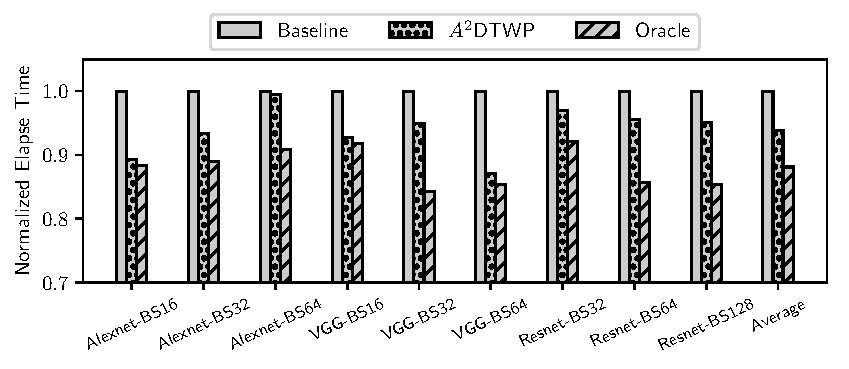
\includegraphics[scale=0.65]{figs/all_bars.pdf}}
    \vspace{-0.2cm}
    \centerline{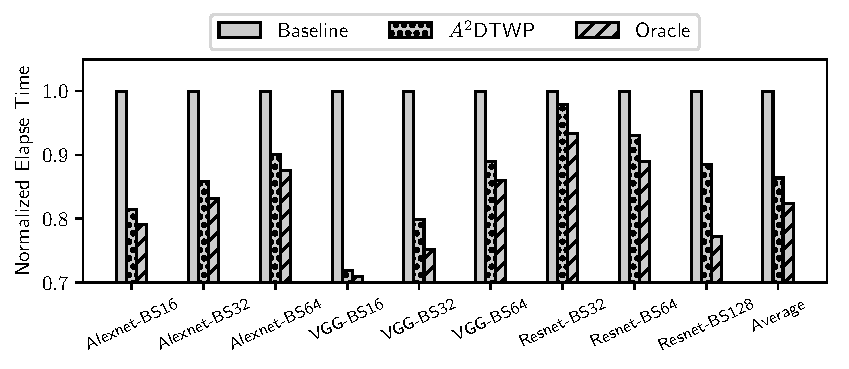
\includegraphics[scale=0.65]{figs/all_bars_p9.pdf}}
    \vspace{-0.5cm}
    \caption{Normalized execution times of the \textit{$A^2$DTWP} and the \textit{oracle} policies with respect to the baseline. 
Results obtained on the x86 system appear in the upper plot while the evalution on the POWER system appears at the bottom.} 
    %\textcolor{cyan}{Average: 
    %$A^2$DtWp 0.938, oracle 0.881}}
    \label{fig:all}
\end{figure}

\subsection{$A^2DTWP$ Performance Profile}
\label{sec:performance}
This section provides a detailed performance profile describing the effects of 
applying $A^2DTWP$ when training the VGG network model with batch size 64 on the x86 and POWER systems described in section~\ref{sec:platform}.
To highlight these effects we also show a performance profile of applying 32-bit 
Floating Point format during training.
The main kernels involved in the training process and their corresponding average execution time in milliseconds are shown in Tables ~\ref{table:performance} and~\ref{table:performance_p9}.
Each kernel can be invoked multiple times by different network layers and it can be overlapped with other operations while processing a batch.
Tables~\ref{table:performance} and~\ref{table:performance_p9} display for all kernels the average execution time of their occurrences within a batch when run on the x96 and the POWER systems, respectively.
%In order to to demonstrate the performance of our $A^2DtWp$ approach, we 
%dissect a typical batch in VGG BS32 (the baseline and the $A^2DtWp$ when 
%ROUNTO=16) into the operations involved and their elapse time in the 
%Table~\ref{table:performance}. 
%Each operation can be invoked multiple times on different layers during a batch 
%and can be overlapped with other operations so we take the average value of all 
%the occurrences in a batch. 
%Nevertheless, it gives an insight look into the efficiency of our approach.

Results appearing in Table~\ref{table:performance} show how time spent transferring 
data from the CPU to the GPU accelerators when applying $A^2DTWP$ on the x86 system, 52.27 ms, 
is significantly smaller than the cost of performing the same operation when using the 32-bit configuration, 153.93 ms. 
This constitutes a 2.94x execution time reduction that compensates the cost of the operations involved in the ADT routine, Bitpack and
Bitunpack, and in the AWP algorithm, the $l^2$-norm computation.
On POWER we observe a similar reduction of 3.20x in the time spent transferring
data from the CPU to the GPUs when applying $A^2DTWP$.
These reductions in terms of CPU to GPU data transfer time are due to a close to 3x reduction in terms of weights size enabled by $A^2DTWP$.
The average execution time of operations where the $A^2DTWP$ technique plays no role remains very similar for the 32-bit Floating Point baseline and $A^2DTWP$ in both systems, as expected.
Tables~\ref{table:performance} and~\ref{table:performance_p9} indicate that performance gains achieved by $A^2DTWP$ are due to data motion reductions, which validates the usefulness of $A^2DTWP$.

Tables~\ref{table:performance} and~\ref{table:performance_p9} also display the overhead associated with AWP and ADT in terms of milliseconds.
The AWP algorithm spends most of its runtime computing the $l^2$-norm of the weights, which takes a total of 3.88 ms within a batch on the x86 system. 
On POWER, the cost of computing the $l^2$-norm of the weights is 0.93 ms.
The other operations carried out by AWP have a negligible overhead.
The two fundamental procedures of ADT are the Bitpack and Bitunpack routines, which take 19.71 and 4.51 ms to run within a single batch on the x86 system.
For the case of POWER, Bitpack and Bitunpack take 10.51 and 1.11 ms, respectively.
Overall, measurements displayed at Table~\ref{table:performance} indicate that AWP and ADT constitute 1.05\% and 6.60\% of the total batch execution time, respectively, on x86.
On the POWER system, AWP and ADT constitute 0.54\% and 6.82\% of the total batch execution time according to Table~\ref{table:performance_p9}. 
Figures ~\ref{alex_improv}, ~\ref{vgg_improv} and ~\ref{fig:all} account for this overhead in the results they display.

\begin{table}
    \caption{Performance profiles of both the $A^2DTWP$ and the 32-bit Floating 
    Point approaches expressed in milliseconds on the x86 system. 
    We consider the VGG network model with batch size 64.} 
    \vspace{-0.35cm}
    \centering
    \begin{tabular}{|P{4.2cm}|P{1.5cm}|P{1.5cm}|}
    \hline
    %\rowcolor{LightCyan}
    & \textbf{32-bit FP} & $\mathbf{A^2DTWP}$\\
    \hline
    %\rowcolor{LightCyan}
    Data Transfer CPU$\rightarrow$GPU& 153.93 & 52.27 \\
    \hline
    %\rowcolor{LightCyan}
    Data Transfer GPU$\rightarrow$CPU& 68.51 & 73.55 \\
    \hline
    %\rowcolor{LightCyan}
    Convolution & 128.72 & 126.13\\
    \hline
    %\rowcolor{LightCyan}
    Fully-connected & 33.51 & 34.17 \\
    \hline
    %\rowcolor{LightCyan}
    Gradient update & 54.39 & 52.86\\
    \hline
    %\rowcolor{LightCyan}
    AWP ($l^2$-norm) & N/A & 3.88 \\
    \hline
    %\rowcolor{LightCyan}
    ADT (Bitpack) & N/A & 19.71 \\
    \hline
    %\rowcolor{LightCyan}
    ADT (Bitunpack) & N/A & 4.51 \\
    \hline
    \end{tabular}
    \label{table:performance}
\end{table}

\begin{table}
    \caption{Performance profiles of both the $A^2DTWP$ and the 32-bit Floating 
    Point approaches expressed in milliseconds on the POWER system. 
    We consider the VGG network model with batch size 64.} 
    \vspace{-0.35cm}
    \centering
    \begin{tabular}{|P{4.2cm}|P{1.5cm}|P{1.5cm}|}
    \hline
    & \textbf{32-bit FP} & $\mathbf{A^2DTWP}$ \\
    \hline
    Data Transfer CPU$\rightarrow$GPU& 39.12 & 12.21 \\
    \hline
    Data Transfer GPU$\rightarrow$CPU& 17.34 & 17.87 \\
    \hline
    Convolution & 69.78 & 71.21\\
    \hline
    Fully-connected & 12.66 & 13.51 \\
    \hline
    Gradient update & 41.29 & 42.98\\
    \hline
    AWP ($l^2$-norm) & N/A & 0.93 \\
    \hline
    ADT (Bitpack) & N/A & 10.51 \\
    %Bitpack & N/A & 10.51 \\
    \hline
    ADT (Bitunpack) & N/A & 1.11 \\
    %Bitunpack & N/A & 1.11 \\
    \hline
    \end{tabular}
    \label{table:performance_p9}
\end{table}

\subsection{Experiments with ImageNet1000}
\label{sec:ImageNet1000}
%We run experiments considering ImageNet1000 to confirm they display the same trends as results shown in Sections~\ref{sec:alexnet}, ~\ref{sec:VGG}, ~\ref{sec:Resnet}, ~\ref{sec:Average}, and ~\ref{sec:performance}, which consider ImageNet200.
We run experiments considering ImageNet1000 to confirm they display the same trends as executions with ImageNet200. 
Network parameters are the same as the ones described in Section~\ref{sec:setup}.
$AWP$ parameters are the ones described in Section~\ref{sec:evaluation1}.
The experimental setup of the evaluation considering ImageNet1000 is the same as the one we use for ImageNet200.
We consider batch sizes that produce the fastest 32-bit FP training for each one of the network models: 64, 64, and 128 for Alexnet, VGG and Resnet, respectively.


Figure~\ref{fig:ImageNet1000} displays results corresponding to the experimental campaign with ImageNet1000 on the x86 system.
In the x-axis we display different epoch counts for each one of the three models: 4, 8, 12, 16, and 20 epochs for Alexnet; 2, 4, 6, and 8 for VGG; and 4, 8, 12, and 16 epochs for Resnet.
The y-axis displays the normalized elapsed time of \textit{$A^2$DTWP} with respect to the the 32-bit Floating Point \textit{baseline} per each model and epoch count.
For the case of Alexnet with batch size 64, \textit{$A^2$DTWP} is slightly faster than the \textit{baseline} as it displays a normalized execution time of 0.995, 0.992, 0.992, 0.996, and 0.990 after 4, 8, 12, 16 and 20 epochs, respectively.
Figure~\ref{fig:all} also reports small gains for the case of Alexnet with batch size 64, which confirms that experiments with ImageNet1000 show very similar trends as the evaluation with ImageNet200.
When applying \textit{$A^2$DTWP} to VGG with 64 batch size, it displays a normalized execution time of 0.907, 0.920, 0.936, and 0.932 with respect to the \textit{baseline} after running 2, 4, 6 and 8 training epochs, respectively.
For the Resnet example, we observe normalized execution times of 0.765, 0.770, 0.778, and 0.777 for \textit{$A^2$DTWP} after 4, 8, 12, and 16 training epochs, respectively,
which constitutes a significant performance improvement.

\begin{figure}%[!bhtp]
    \centerline{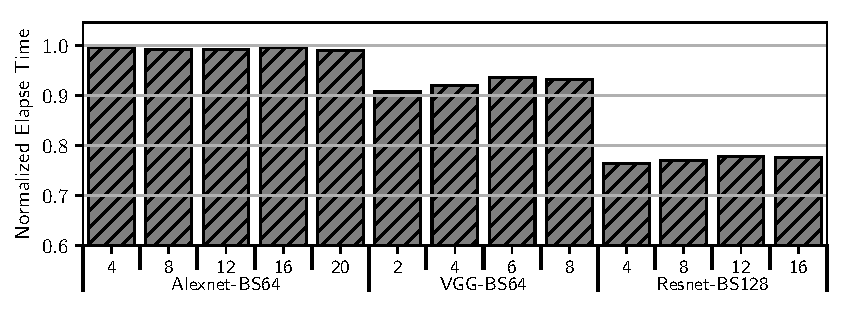
\includegraphics[scale=0.65]{figs/imagenet-1k-3net.pdf}}
    \caption{Normalized execution time of \textit{$A^2$DTWP} with respect to \textit{baseline} considering the Imagenet1000 data set. Training for Alexnet, VGG and Resnet considers up to 20, 8, and 16 epochs, respectively.}
    %\vspace{-0.5cm}
    \label{fig:ImageNet1000}
\end{figure}

In terms of validation error, both \textit{$A^2$DTWP} and \textit{baseline} display very similar top-5 values at the end of each epoch.
%For example, for the case of VGG, the Floating Point 32-bit \textit{baseline} approach displays validation errors of 88.04\%, 64.02\%, 56.46\%, and 46.18\% after 2, 4, 6, and 8 training epochs. 
%\textit{$A^2$DTWP} achieves validation errors of 89.97\%, 67.12\%, 55.99\%, and 46.89\% for the same epoch counts.
For example, for the case of VGG, the Floating Point 32-bit \textit{baseline} approach displays a validation error of 88.04\% after 2 training epochs while \textit{$A^2$DTWP} achieves a validation error of 89.97\% for the same epoch count, that is, an absolute difference of 1.93\%.
After 4, 6, and 8 training epochs absolute distances of top-5 validation errors between \textit{$A^2$DTWP} and \textit{baseline} are 3.09\%, 0.47\%, and 0.71\%, respectively.
Top-5 validation error keeps decreasing in an analogous way for both \textit{baseline} and \textit{$A^2$DTWP} as training goes over more epochs, although \textit{$A^2$DTWP} is significantly faster.
Our evaluation indicates that \textit{$A^2$DTWP} can effectively accelerate training while achieving the same validation error as the 32-bit FP \textit{baseline} when considering ImageNet1000.

%\subsection{$A^2DTWP$ Data Movement Reduction}
%Table~\ref{table:transfer} shows the avergage data movement in MB between the CPU 
%host and GPUs at the beginning of each batch on the POWER system on three 
%particular networks, Alexnet-BS32, VGG-BS32 and Resnet-BS128. The $A^2DTWP$ 
%reduces the data movement by 19.38\%, 24.8\% and 15.94\% respectively.
%
%\begin{table}[H]
%    \caption{Average data transfer per batch on the POWER system (MB)}
%    \vspace{-0.35cm}
%    \centering
%    \begin{tabular}{|P{4.2cm}|P{1.5cm}|P{1.5cm}|}
%    \hline
%    & \textbf{32-bit FP} & $\mathbf{A^2DTWP}$\\
%    \hline
%    Alexnet-BS32 & 98.63 & 79.81 \\ %19.38
%    \hline
%    VGG-BS32 & 387.92 & 291.54 \\ %24.8
%    \hline
%    Resnet-BS128 & 69.05 & 58.07 \\ %15.94
%    \hline
%    \end{tabular}
%    \label{table:transfer}
%\end{table}


%\subsection{Analysis of Weights' Dynamic Range}
%\label{sec:histograms}
%This section describes the weights' dynamic range of VGG's 9th layer by showing its distribution of weights' values at different points of the training process. 
%Figure~\ref{fig:hist} plots four different distributions corresponding to 0\%, 50\%, 75\% and 100\%, respectively, of VGG's training process with the batch size parameter set to 64.
%These distributions are generated with the 32-bit floating point precision.
%We can see in Figure~\ref{fig:hist} how the initial distribution of weights is randomly generated. % over the interval $[-0.27;0.27]$.
%As training progresses there is an increasing amount of weights with values very close to $0$
%, which is a trend observed for most of the layers of the VGG, the Alexnet and the Resnet models.
%What explains the usefulness of our approach is the fact that during the initial stages of the training process weight's values are far from the final ones. 
%As training progresses, weights values become closer to their final ones and more accuracy is required to keep adjusting them.
%\begin{figure}%[!bhtp]
%    \centerline{
%        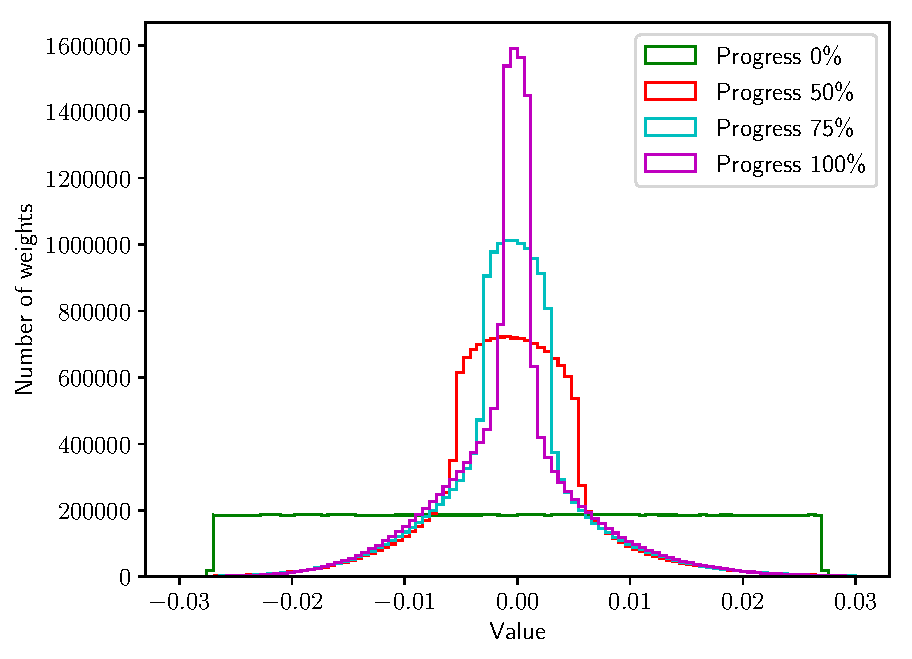
\includegraphics[scale=0.60]{figs/weights_9.pdf}
%    }
%    \vspace{-0.5cm}
%    \caption{Values' weights distribution considering the 9th layer of VGG with BS=64.} 
%    \label{fig:hist}
%    \vspace{-0.3cm}
%\end{figure}

\section{Related work}
\label{sec:Relatedworks}
A rich body of literature exists describing the effects of using  
data representation formats smaller than the 32-bit Floating Point standard while training neural networks. 
Previous work provides theoretical analysis on the  
ability to learn under limited-precision scenarios of simple networks~\cite{holi93}. 
In recent years, researchers have shown that fixed-precision arithmetic is well suited 
for deep neural networks training~\cite{courbariaux14}, particularly when combined with
stochastic rounding~\cite{gupta15}. 
New data representation formats targeting dynamic and low accuracy opportunities for deep learning have been proposed~\cite{flexpoint17}.
While these approaches have a very large potential for reducing DNNs training costs, 
they do not target 
the data movement problem and, as such, they are orthogonal to the approach 
presented by this paper.

There is a methodology for training deep neural models using 16-bit FP numbers without modifying hyperparameters or losing network accuracy~\cite{Micikevicius2018}.
This previous approach avoids losing accuracy by keeping a 32-bit copy of weights,
scaling the loss function to preserve small gradient updates, and
using 16-bit arithmetic that accumulates into single-precision registers.
%The approach we present in this paper also uses different numerical representation.
This previous approach exploits the tolerance of DNN to data representation formats smaller than the 32-bit FP standard, as our proposal does.
However, our goal is fundamentally different since we reduce data motion in the context of heterogeneous high-end architectures while this previous approach aims at reducing the computing and storage costs of DNN training.
This approach can be combined with \textit{$A^2$DTWP} by decompressing network weights to half-precision to reduce GPU computing time.
This reduction would increase the impact of data motion in the overall performance, which imples that the benefits of \textit{$A^2$DTWP} could be evern larger. 

There are several proposals aimed at improving the Stochastic Gradient Descent (SGD) method like the
Asynchronous SGD~\cite{jeff12} and its variants~\cite{hogwild, 
zhang14}. 
Other approaches \cite{coates13, quoc11} exploit 
model parallelism instead of data-level parallelism to orchestrate large-scale parallel executions of deep learning workloads. 
If the different parallel instances of this model-level parallel scheme had 
different precision requirements, it would be possible to apply approaches close to the ones we present in this paper.

Some previous approaches reduce networks storage and energy requirements to run inference  
on mobile devices~\cite{Han15}. 
While these approaches achieve very large storage reductions, they target inference on embedded systems with limited hardware resources.
%Their network compression techniques are too costly for appyling them many times during training with minimal overhead.
Other approaches achieve large gradient compression ratios in the context of distributed training in mobile devices~\cite{Lin18}.
These approaches achieve very remarkable speedups in low network bandwidth environments and
are applied to scenarios that require frequent and costly allreduce communications.
While they are very valuable in the mobile computing arena, the scope of these approaches is not high-performance computing. 

Several approaches target synchronization costs of SGD gradient updates in the context of parallel executions.
They either quantize gradients to ternary levels \{-1, 0, 1\} to
reduce the overhead of gradient synchronization~\cite{sgd0}, or they propose a family of algorithms allowing for lossy
compression of gradients called Quantized SGD (QSGD)~\cite{sgd1}.
Techniques based on sparsifying gradient updates by removing the 
smallest gradients by absolute value~\cite{sgd2} can also reduce SGD synchronization costs.   
While these approaches apply techniques based on small data representation formats to reduce the synchronization costs of SGD gradient updates, \textit{$A^2$DTWP} targets the cost of sending DNNs weights to the GPU accelerators.
Therefore, these approaches are orthogonal to \textit{$A^2$DTWP} and can be combined with it to reduce as much as possible training communication cost. 
In particular, techniques targeting synchronization costs of SGD gradient updates can be used to reduce GPU to CPU data transfer overhead while \textit{$A^2$DTWP} targets CPU to GPU communication cost.
Therefore, the combination of \textit{$A^2$DTWP} with techniques targeting synchronization costs of SGD gradient updates would reduce both CPU to GPU and GPU to CPU communication overhead.

To the best of our knowledge, this paper is the first in accelerating the training of deep neural networks in multi-GPU high-end systems by reducing data motion.
Our method combines the use of an 
algorithm to dynamically change DNNs weights data representation format during 
training with a highly tuned data compression and decompression procedure. 
Our solution successfully reduces data motion and achieves a significant performance improvement on cutting-edge high-end systems.
While there are previous proposals exploiting mixed precision scenarios to accelerate training, they are orthogonal to our approach as they speed up arithmetic and reduce memory footprint.
Importantly, our proposal can be combined with these previous approaches to obtain a highly optimized training method that minimizes data transfers and accelerates arithmetic in the context of multi-GPU systems. 
%Using this kind of nodes for DNN training is becoming a very common practice in the parallel computing context~\cite{You17}.


\section{Conclusion}
\label{sec:conclusion}

This paper proposes $A^2DTWP$, which reduces data movement 
across heterogeneous environments composed of several GPUs and multicore CPU devices 
in the context of deep learning workloads.
The $A^2DTWP$ framework is composed of the AWP algorithm and the ADT procedure.
AWP is able to dynamically define the weights data representation format
during training. 
This paper demonstrates that AWP is
effective without any deterioration on the learning capacity of
the neural network.
To transform AWP decisions into real performance gains, 
we introduce the ADT procedure, which efficiently compresses network's weights before sending them to the GPUs. 
This procedure exploits both thread- and SIMD-level parallelism. 
By combining AWP with ADT we are able to achieve a significant performance gain 
when training network models such as Alexnet, VGG or Resnet.
Our experimental campaign considers different batch sizes and two different multi-GPU high-end systems.

This paper is the first in proposing a solution that relies on  
reduced numeric data formats to mitigate the cost of sending DNNs weights to 
different hardware devices during training.
While our evaluation targets heterogeneous high-end systems composed of several GPUs 
and CPU multicore devices, techniques presented by this paper are easily generalizable 
to any context involving several hardware accelerators exchanging large 
amounts of data.
Taking into account the prevalence of deep learning-specific accelerators in large
production systems~\cite{Jouppi2017}, the contributions of this paper are 
applicable to a wide range of scenarios involving different kinds of accelerators.


%\input{sec_acknowledgments} % TO BE COMMENTED IN BLIND SUBMISSION
%\newpage

%\bibliographystyle{ACM-Reference-Format}
\balance
\bibliography{references}

\end{document}
